\documentclass[10pt]{article}
\ifdefined\papreprint
\usepackage[preprint]{tmlr}
\else
\usepackage{tmlr}
\fi

% ---------- Mathematics ----------
\usepackage{amsmath}
\usepackage{amssymb}
\usepackage{booktabs}
\usepackage{tabularx}
\usepackage{array}
\usepackage{enumitem}

% ---------- Figures ----------
\usepackage{graphicx}
\usepackage{float}
\usepackage{needspace}
\usepackage[section]{placeins}
\usepackage{flafter}
\usepackage{tikz}
\usetikzlibrary{positioning,arrows.meta,fit,calc}

% ---------- Typography ----------
\usepackage[T1]{fontenc}
\usepackage{lmodern}
\usepackage{microtype}
\usepackage{pgfplots}
\pgfplotsset{compat=1.18}
\usepackage{xurl}
\usepackage[hidelinks]{hyperref}
\hypersetup{
  pdftitle={One Vector from Many: Hierarchical Long-Document Representation through Recursive Geodesic Transformer Composition},
  pdfauthor={},
  pdfsubject={Recursive composition of frozen text representations; clean-v6 study}
}
\usepackage[
    font=small,
    labelfont=bf,
    labelsep=colon
]{caption}


% Helps avoid ugly line overflow without globally using \sloppy
\emergencystretch=1.5em

\newcolumntype{Y}{>{\raggedright\arraybackslash}X}
\newcolumntype{C}{>{\centering\arraybackslash}X}

\title{One Vector from Many: Hierarchical Long-Document Representation through Recursive Geodesic Transformer Composition}

\author{
\name Mihnea-Teodor Stoica\\
\addr International Computer High School of Bucharest
}

\date{September 2026}

\begin{document}

\maketitle

\begin{abstract}
Splitting a long document into chunks produces multiple embeddings where a
system may need one. We study how to merge these embeddings into a vector
in the frozen encoder's output space that can itself be reused in further
merges. Our geodesic Transformer combines up to four adjacent representations
at a time, whether they encode original chunks or previously merged spans.
Each merge preserves the embedding dimension and unit-sphere domain and
propagates the exact token count. Its output can enter the same operator
without conversion; teacher supervision trains it to approximate the encoder's
direct embedding of the combined text. On 4,000 document
prefixes of 1,025--4,096 tokens, a single merge achieves mean cosine similarity
\(0.9850\) to a GTE-ModernBERT-based teacher, compared with \(0.9829\)
for token-weighted averaging,
across three checkpoints. This small gain costs approximately \(110\times\)
as much in measured batched composition, excluding text encoding. Recursive
reuse tests show sensitivity to tree structure and chunk boundaries, and four
retrieval tasks show no consistent advantage over averaging. The method thus
provides recursively reusable embeddings in the same geometric domain, with
empirical rather than guaranteed semantic alignment.
\end{abstract}

\section{Introduction}

A text embedding maps an input passage to a fixed-dimensional vector, allowing
systems to compare or retrieve passages using vector similarity
\cite{reimers-gurevych-2019-sentence}. An encoder has a bounded context window,
so a long document may need to be split into chunks and encoded separately
\cite{gunther-etal-2023-jina-embeddings-2,dai-etal-2022-revisiting}. This leaves
a sequence of chunk vectors rather than the single document vector that some
downstream systems require. Our goal is to make those embeddings composable:
merging several should yield another embedding in the original encoder's
output space, usable as an input to subsequent merges. The encoder remains
unchanged, or \emph{frozen}; composition should not require a new representation
space or a separate conversion between successive merges.

The proposed merger takes two to four adjacent embeddings and produces a
\emph{parent} representing their combined text. It accepts parents as well as
original chunk embeddings, allowing the same learned operation to build a
single document vector through successive merges. Each parent retains the
original embedding dimension and unit norm, together with the exact number of
tokens it represents. Thus, a merged representation has the same interface as
the representations from which it was built.

Here, remaining in the \emph{same geometric space} means retaining the encoder's
output coordinates, dimensionality, unit-sphere domain, and cosine comparison
rule, rather than producing a code in a separate latent space. Supervision aims to align the output with the encoder's representation of
the combined span; the geometric construction alone does not guarantee that
alignment (Section~\ref{sec:problem}).

Flat token-weighted averaging is a simple alternative. Reproducing it exactly
through recursive aggregation requires retaining the unnormalized weighted
sum, or equivalent magnitude information, rather than only a normalized
vector and token count. Reusability alone does not establish an advantage for
learning; we test whether learned weighting and a bounded spherical correction
produce a more faithful parent.
Unlike approaches that extend the encoder's context or jointly encode the
document hierarchy
\cite{beltagy-etal-2020-longformer,zaheer-etal-2020-bigbird,zhang-etal-2019-hibert,wu-etal-2021-hi},
our method operates on embeddings that have already been computed.

To measure that fidelity, we use spans that the frozen encoder can process
directly. Its embedding of the combined span is the \emph{teacher target},
and we compare both the learned merger and token-weighted averaging with that
target. Direct fidelity is measured on short, one-merge prefixes; recursive
robustness and longer-document utility are evaluated separately. The primary
comparison asks whether learning improves agreement with the encoder and at
what composition cost. Because documents longer than the encoder's context
lack a direct teacher target, complete-document runs measure execution and
retrieval. Supporting checks vary chunk boundaries and reduction trees and
test whether a parent allows reconstruction of its input embeddings.

We present and evaluate (i) a shared merger whose outputs can be reused as inputs
while retaining the frozen encoder's embedding dimension and unit norm and
propagating exact token counts; (ii) a bounded spherical correction trained for
teacher alignment, with auxiliary parent-only reconstruction; and (iii) an
evaluation separating this structural reusability from semantic fidelity,
recursive robustness, constituent reconstruction, downstream utility, and cost.
Section~\ref{sec:problem} formalizes the task, Section~\ref{sec:method}
describes the model, and Section~\ref{sec:experimental-setup} defines the
comparisons used to evaluate it.

\section{Related Work}

\subsection{Long-Context and Hierarchical Document Encoding}

Sparse-attention Transformers and long-context embedding models extend the
text that can be processed directly, while hierarchical methods encode smaller
units before combining their representations
\cite{beltagy-etal-2020-longformer,zaheer-etal-2020-bigbird,gunther-etal-2023-jina-embeddings-2,dai-etal-2022-revisiting}.

Hierarchical Attention Networks and HIBERT model textual units at multiple
levels \cite{yang-etal-2016-hierarchical,zhang-etal-2019-hibert}.
Hi-Transformer encodes sentences independently, processes their representations
with a document-level Transformer, and feeds document context back into sentence
modeling before hierarchical pooling \cite{wu-etal-2021-hi}. Its global
attention acts on fewer units than token-level attention, but remains
\(O(N^2)\) in the number of sentence representations. Dai et al. compare
hierarchical and sparse-attention approaches for long-document classification,
including the effects of splitting strategy \cite{dai-etal-2022-revisiting}.

\subsection{Chunk-Level Representation Learning}

Chunk-level methods can change either the context available to a chunk or the
training objective of the encoder. Late Chunking encodes a longer text before
pooling token representations within chunk boundaries, allowing each chunk
embedding to incorporate surrounding context
\cite{gunther-etal-2024-late-chunking}. The Chunk Prediction Encoder instead
learns document representations by predicting a held-out chunk contrastively
and whether a candidate chunk belongs to the document
\cite{abro-etal-2026-learning}. Both address representation learning upstream
of the combination problem studied here.

\subsection{Recursive and Geometry-Aware Composition}

Recursive models build representations of larger textual units from smaller
ones. Tree-LSTM supports tree-structured composition, while Gumbel Tree-LSTM
learns task-specific tree structures from text
\cite{socher-etal-2013-recursive,tai-etal-2015-improved,choi-etal-2018-learning}.
Pandey uses syntax-guided neural modules to approximate Transformer sentence
embeddings, probing whether their representations admit compositional
explanations \cite{pandey-2023-syntax}. Our focus is instead a shared operation
that can repeatedly combine adjacent document chunks without a syntactic parse.

Directional comparisons such as cosine similarity also motivate composition
methods that respect embedding geometry. Spherical Text Embedding learns word
and paragraph vectors on the unit hypersphere using Riemannian optimization
\cite{meng-etal-2019-spherical}. GeoGNN studies semantic drift when aggregating
pretrained text representations in graphs, using logarithmic and exponential
maps to aggregate through tangent spaces \cite{yang-etal-2025-geognn}.
These methods motivate our spherical parameterization; whether it preserves
useful information remains an empirical question.

\section{Problem Formulation}
\label{sec:problem}

Let \(D\) denote a document, and let \(g\) be a pretrained, frozen text encoder with a maximum context length. The document \(D\) may exceed this context length, so \(g\) cannot encode it in a single forward pass. We therefore partition \(D\) into an ordered sequence of \(N\) chunks,

\[
C = (c_1, c_2, \ldots, c_N),
\]

where each chunk \(c_i\) fits within the context window of \(g\). Here
\(g\) denotes the complete frozen representation procedure, including the
specified pooling and normalization, rather than the backbone alone. We call
this procedure the \emph{teacher}: when a complete span fits within its usable
context, its directly encoded embedding provides a target for composition.

We encode each chunk independently using the same encoder \(g\):

\[
e_i = g(c_i), \qquad e_i \in \mathbb{R}^d,
\]

where \(d\) is the dimensionality of the embedding space. The document is therefore initially represented by the ordered sequence

\[
E = (e_1, e_2, \ldots, e_N).
\]

For each chunk \(c_i\), let \(n_i \in \mathbb{N}_{>0}\) denote its number of tokens. Each representation is therefore associated with a pair \((e_i,n_i)\), consisting of its embedding and the number of tokens represented by that embedding.

We seek a learned composition operator that acts on an ordered group of \(k\in\{2,3,4\}\) representations. We call the inputs \emph{children} and their combined output a \emph{parent}; the arity \(k\) is the number of children in a merge. For each supported arity \(k\),

\[
f_\theta :
(\mathbb{R}^d \times \mathbb{N}_{>0})^k
\rightarrow
\mathbb{R}^d \times \mathbb{N}_{>0},
\qquad
k\in\{2,3,4\}.
\]

Given an ordered group

\[
\big((e_1,n_1),\ldots,(e_k,n_k)\big),
\]

the operator produces

\[
f_\theta\big((e_1,n_1),\ldots,(e_k,n_k)\big)
=
\left(
e_{\mathrm{parent}},
\sum_{i=1}^{k}n_i
\right),
\]

where \(e_{\mathrm{parent}}\in\mathbb{R}^d\) represents the combined span of the ordered inputs.

Because \(e_{\mathrm{parent}}\) has the same dimensionality as the original chunk embeddings and remains paired with the exact number of tokens it represents, the output of one composition can be used as an input to another. The same shared operator can therefore be applied recursively to contiguous groups of representations, progressively reducing the ordered sequence until a single pair remains,

\[
(e_D,n_D),
\qquad
n_D=\sum_{i=1}^{N} n_i,
\]

where \(e_D \in \mathbb{R}^d\) is the resulting document representation.

The central requirement is closure of the representation interface under
composition: a parent must have the same embedding dimension and unit norm as
a child and carry its represented token count, so it can enter the next merge
without conversion. Section~\ref{sec:geodesic} gives the spherical construction
and its assumptions. This is not closure of the encoder's set of attainable
semantic representations, nor a claim that composition is associative.
We train \(f_\theta\) to make these reusable parents approximate the frozen
encoder's direct representations wherever teacher targets are available;
the experiments assess how well that alignment survives recursive reuse.

\section{Method}
\label{sec:method}

The merger starts from a weighted average of normalized child embeddings and
learns a bounded change in its direction. A shared network predicts both the
weights and this directional correction. The same merger is reused at every
level of the document tree; a separate decoder supplies reconstruction
supervision during training but is not needed to compose a document.

\subsection{Model Architecture}
\label{sec:model-architecture}

The composition model is a shared four-way merger, denoted K4, with four input slots. The first \(k\in\{2,3,4\}\) slots contain the ordered child embeddings \(e_i\in\mathbb{R}^{768}\) and positive token counts \(n_i\); these form the active prefix of the slots, not a prefix of the document. Trailing inactive slots are padded and masked, and their contextual states are set to zero before the four positions are flattened. Each embedding is L2-normalized \cite{meng-etal-2019-spherical},

\[
x_i=\frac{e_i}{\lVert e_i\rVert_2},
\]

and its relative token mass, the fraction of represented tokens belonging to that child, is

\[
q_i=\frac{n_i}{\sum_{j=1}^{k}n_j}.
\]

For each child, the model forms

\[
u_i=[x_i;\,q_i;\,\log(\max(q_i,\epsilon))]\in\mathbb{R}^{770}.
\]

Here \(\epsilon=10^{-8}\) is a numerical stabilizer. A shared linear projection, LayerNorm, and GELU map \(u_i\) to dimension \(1024\); a learned slot embedding then encodes child order.

The resulting sequence is processed by an eight-layer norm-first Transformer encoder \cite{vaswani-etal-2017-attention,xiong-etal-2020-layernorm} with 16 attention heads, model dimension \(1024\), feed-forward dimension \(3072\), GELU activation \cite{hendrycks-gimpel-2016-gelu}, and dropout \(0.05\) \cite{srivastava-etal-2014-dropout}. A salience head applies LayerNorm \cite{ba-etal-2016-layernorm} and produces

\[
\delta_i=\tanh\!\left(W_s\operatorname{LayerNorm}(h_i)+b_s\right)
\]

from each active contextual state \(h_i\). This salience correction adjusts the
child's contribution relative to its token mass.

The four contextual states are flattened and concatenated with the spherical reference representation \(a\), the normalized weighted average defined in Section~\ref{sec:geodesic}. The resulting 4864-dimensional vector is processed by a two-layer trunk,

\[
4864\rightarrow3072\rightarrow3072,
\]

with LayerNorm, GELU activations, and dropout \(0.05\). A zero-initialized linear direction head then produces a raw correction vector \(r\in\mathbb{R}^{768}\).

The merger contains 111,538,433 trainable parameters; the strict decoder adds
12,077,825. Appendix~\ref{app:parameter-accounting} gives the component breakdown.
The wider 1,152-dimensional K4 control did not improve the selected system
(Section~\ref{sec:architecture-scaling}).

\begin{figure}[!t]
\centering

\definecolor{cblue}{RGB}{224,236,248}
\definecolor{cyellow}{RGB}{252,239,204}
\definecolor{cgreen}{RGB}{224,240,225}
\definecolor{cred}{RGB}{248,226,226}
\definecolor{cgray}{RGB}{245,245,245}

\resizebox{!}{0.50\textheight}{%
\begin{tikzpicture}[
>=Latex,
wide/.style={draw=black!65,rounded corners=2pt,line width=.65pt,minimum width=8.6cm,minimum height=8.5mm,align=center,inner sep=3pt,font=\small},
mid/.style={draw=black!65,rounded corners=2pt,line width=.65pt,minimum width=6.4cm,minimum height=8.5mm,align=center,inner sep=3pt,font=\small},
smallbox/.style={draw=black!60,rounded corners=2pt,line width=.55pt,minimum width=1.75cm,minimum height=8.5mm,align=center,inner sep=2pt,font=\scriptsize},
flow/.style={-{Latex[length=2mm,width=1.3mm]},line width=.8pt,draw=black!75},
aux/.style={-{Latex[length=1.8mm,width=1.2mm]},line width=.6pt,draw=black!50},
meta/.style={-{Latex[length=1.8mm,width=1.2mm]},dashed,line width=.65pt,draw=black!55}
]

% Output
\node[mid,fill=cred] (parent) {
    \textbf{Parent representation}\\[-1mm]
    \(e_{\mathrm{parent}}\in\mathbb{R}^{768}\),\qquad
    \(n_{\mathrm{parent}}=\sum_i n_i\)
};

% Geodesic path
\node[mid,fill=cgreen,below=5mm of parent] (geo) {
    \textbf{Geodesic composition}\\[-1mm]
    tangent projection \(\rightarrow\) bounded correction \(\rightarrow\exp_a\)
};
\draw[flow] (geo) -- (parent);

\node[mid,fill=cgreen,below=5mm of geo] (direction) {
    \textbf{Direction head}\\[-1mm]
    \(r\in\mathbb{R}^{768}\)
};
\draw[flow] (direction) -- (geo);

\node[wide,fill=cgreen,below=5mm of direction] (trunk) {
    \textbf{Trunk}\\[-1mm]
    \([h_1;h_2;h_3;h_4;a]\)\qquad
    \(4864\rightarrow3072\rightarrow3072\)
};
\draw[flow] (trunk) -- (direction);

% Reference construction
\node[mid,fill=cyellow,below=5mm of trunk] (anchor) {
    \textbf{Spherical reference}\\[-1mm]
    \(a=\operatorname{normalize}\!\left(\sum_i w_i x_i\right)\)
};
\draw[flow] (anchor) -- (trunk);

\node[mid,fill=cyellow,below=4.5mm of anchor] (weights) {
    \textbf{Composition weights}\\[-1mm]
    \(w_i=\operatorname{softmax}_i(\log q_i+\delta_i)\)
};
\draw[flow] (weights) -- (anchor);

\node[mid,fill=cyellow,below=4.5mm of weights] (salience) {
    \textbf{Semantic-salience head}\\[-1mm]
    \(h_i\rightarrow\delta_i\)
};
\draw[flow] (salience) -- (weights);

% Contextualization
\node[wide,fill=cblue,below=5mm of salience] (states) {
    \textbf{Contextual child states}\\[-1mm]
    \(h_1\qquad h_2\qquad h_3\qquad h_4\)
};
\draw[flow] (states) -- (salience);
\draw[aux] (states.east) -- ++(11mm,0) |- (trunk.east);

\node[wide,fill=cblue,below=5mm of states] (transformer) {
    \textbf{Transformer encoder}\\[-1mm]
    8 layers\qquad 16 heads\qquad
    \(d_{\mathrm{model}}=1024\)\qquad \(d_{\mathrm{FF}}=3072\)
};
\draw[flow] (transformer) -- (states);

\node[wide,fill=cblue,below=5mm of transformer] (features) {
    \textbf{Shared child feature encoding}\\[.5mm]
    \(x_i=\dfrac{e_i}{\lVert e_i\rVert_2}\)\qquad
    \(q_i=\dfrac{n_i}{\sum_j n_j}\)\qquad
    \(\log(\max(q_i,\epsilon))\)\\[.5mm]
    shared \(770\rightarrow1024\) projection + learned slot embedding
};
\draw[flow] (features) -- (transformer);
\draw[aux] (features.west) -- ++(-11mm,0) |- (anchor.west);

% Ordered child slots
\coordinate (slots) at ($(features.south)+(0,-11mm)$);
\node[smallbox,fill=cgray] (c1) at ($(slots)+(-3.15cm,0)$) {
    \textbf{Slot 1}\\ \((e_1,n_1)\)
};
\node[smallbox,fill=cgray] (c2) at ($(slots)+(-1.05cm,0)$) {
    \textbf{Slot 2}\\ \((e_2,n_2)\)
};
\node[smallbox,fill=cgray] (c3) at ($(slots)+(1.05cm,0)$) {
    \textbf{Slot 3}\\ \((e_3,n_3)\)
};
\node[smallbox,fill=cgray] (c4) at ($(slots)+(3.15cm,0)$) {
    \textbf{Slot 4}\\ \((e_4,n_4)\)
};

\coordinate (f1) at ($(features.south west)!0.20!(features.south east)$);
\coordinate (f2) at ($(features.south west)!0.40!(features.south east)$);
\coordinate (f3) at ($(features.south west)!0.60!(features.south east)$);
\coordinate (f4) at ($(features.south west)!0.80!(features.south east)$);
\draw[flow] (c1.north) -- ++(0,3mm) -| (f1);
\draw[flow] (c2.north) -- ++(0,3mm) -| (f2);
\draw[flow] (c3.north) -- ++(0,3mm) -| (f3);
\draw[flow] (c4.north) -- ++(0,3mm) -| (f4);

\node[font=\scriptsize,text=black!60,below=2mm of c2.south east,anchor=north] {
    ordered active prefix \(k\in\{2,3,4\}\); trailing slots are masked
};

% Exact structural count path
\node[font=\scriptsize,text=black!60,right=5mm of c4] (countmeta) {
    exact counts \(n_1,\ldots,n_k\)
};
\draw[meta] (countmeta.east) -- ++(8mm,0) |- (parent.east);

\end{tikzpicture}%
}

\caption{Architecture of the shared composition model. Solid arrows denote learned embedding transformations; thin solid arrows denote auxiliary inputs, and the dashed path denotes exact token-count propagation.}
\label{fig:model-architecture}
\end{figure}

\Needspace{8\baselineskip}
\subsection{Geodesic Composition}
\label{sec:geodesic}

Because the embeddings are normalized, the composition can be expressed as a
movement on the unit sphere. The reference gives a starting direction; a
geodesic correction moves along a great-circle arc to the parent direction.

The salience corrections modify the token-mass prior to produce the composition weights

\[
w_i=\operatorname{softmax}_i(\log q_i+\delta_i).
\]

These weights define the normalized spherical reference representation

\[
a=\operatorname{normalize}\!\left(\sum_{i=1}^{k}w_i x_i\right).
\]

The raw direction \(r\) is projected onto the tangent space of the unit sphere at \(a\):

\[
v=r-(a^\top r)a.
\]

Writing \(\rho=\lVert v\rVert_2\), its magnitude is smoothly bounded to \(0.5\) radians:

\[
\tilde v=
\begin{cases}
\dfrac{0.5\tanh(\rho/0.5)}{\rho}\,v,&\rho>0,\\[6pt]
0,&\rho=0.
\end{cases}
\]

Finally, with \(\alpha=\lVert\tilde v\rVert_2\), the parent embedding is obtained using the exponential map on the unit sphere:

\[
e_{\mathrm{parent}}=
\begin{cases}
\displaystyle
\cos(\alpha)a+\sin(\alpha)\frac{\tilde v}{\alpha},
&\alpha>0,\\[6pt]
a,&\alpha=0.
\end{cases}
\]

Thus, the network predicts a bounded geodesic correction to the spherical
reference rather than an unconstrained parent. This is the exponential map on
the unit sphere \cite{absil-etal-2008-manifolds}. For a nonzero weighted reference
and exact arithmetic, \(a^\top\tilde v=0\),
\(\lVert e_{\mathrm{parent}}\rVert_2=1\), and its geodesic distance from
\(a\) is \(\alpha<0.5\). These are geometric properties, not guarantees of
semantic fidelity or distribution matching. The implementation uses stable
limiting forms at zero; the zero-initialized direction head initially returns
the reference exactly. In the continuation training used here, the merger
instead loads already-trained parameters (Section~\ref{sec:training-configuration}). Appendix~\ref{app:geometry} relates this parameterization to a normalized
tangent residual.

\subsection{Recursive Aggregation}
\label{sec:recursive-aggregation}

The recursive reduction begins from an ordered sequence of nodes, where each node consists of an embedding and an exact positive token count. At the leaf level, these nodes correspond to contiguous, non-overlapping document chunks; at later levels, they may represent spans produced by previous merges. At each reduction level, the sequence is scanned from left to right and divided into contiguous groups of at most four nodes. Full groups of four are merged first; a final remainder of two or three nodes is merged as a smaller active prefix, while a final singleton is carried forward unchanged. Child order is preserved within every group, and every actual merge uses the same shared model parameters.

For a group of children with token counts \(n_1,\ldots,n_k\), the resulting parent count is the exact sum
\[
n_{\mathrm{parent}}=\sum_{i=1}^{k}n_i.
\]
Token counts therefore remain structural metadata and are not predicted by the model. At subsequent levels, the relative token masses \(q_i\) reflect the number of original tokens represented by each recursive child rather than assigning equal structural mass to all children.

The parent embeddings produced at one level, together with any carried singleton, form the ordered sequence for the next level. Because every parent embedding has the same 768-dimensional form as the original leaf embeddings, the same merger can be applied again without changing the architecture. Contiguous reduction is repeated until a single root embedding remains, which serves as the document-level representation. The reduction rule has no fixed token, leaf-count, or depth cap. Actual
execution remains bounded by resources and finite-precision arithmetic; the
empirical scale is reported in Section~\ref{sec:full-results}.

For fixed model dimensions and maximum arity four, reduction requires
\(O(N)\) merge operations and \(O(\log N)\) sequential levels
(derivation in Appendix~\ref{app:merge-complexity}). This excludes leaf
encoding and does not imply an efficiency advantage over
flat pooling, which is also linear in the number of leaves. The learned
operator is order-sensitive and is not constrained to be associative, so its
output is specific to the stated segmentation and reduction tree.

\subsection{Strict Parent-Only Decoder}
\label{sec:strict-decoder}

To encourage the parent to retain information about its constituents, a
training-time decoder predicts the ordered child embeddings from the parent
alone. Strict parent-only means that no child-specific inputs or metadata
are supplied to it. For a generated parent \(z\), let
\(p=\operatorname{normalize}(z)\). A learned linear projection
\(W_p p+b_p\in\mathbb{R}^{1024}\) is repeated across four slots and combined
with learned slot embeddings. A single norm-first Transformer layer, with
16 heads, a 3072-dimensional feed-forward block, GELU, and dropout \(0.05\),
produces slot states \(u_i^{\mathrm{dec}}\). Shared linear heads yield child
residuals and importance logits:
\begin{align}
 b_i &= \frac{0.25}{\sqrt d}\tanh\!\left(W_c u_i^{\mathrm{dec}}+b_c\right),
 & \hat{x}_i &= \operatorname{normalize}(p+b_i),\label{eq:strict-decoder}\\
 \ell_i &= W_w u_i^{\mathrm{dec}}+b_w,
 & \hat{w}_i &= \operatorname{softmax}_i(\ell_i),\qquad d=768.
\end{align}
Both output heads are zero-initialized: before decoder training, every child
prediction equals the parent and importance weights are uniform. The decoder
always returns four slots; it receives neither the active arity nor an
oracle mask indicating which slots are active. Evaluation masks inactive target slots outside the decoder.

The bounded residual restricts every prediction to a neighborhood of the
parent. Since \(\lVert b_i\rVert_2\leq0.25\), its angular distance from
\(p\) is at most \(\arcsin(0.25)\approx14.48^\circ\), as derived in
Appendix~\ref{app:geometry}. This architectural restriction must be considered
when interpreting reconstruction scores: the decoder cannot produce arbitrary
child directions, regardless of what the parent encodes.

\subsection{Training Objectives}
\label{sec:training-objectives}

The merger is trained to match the frozen teacher wherever a valid direct target exists. Let \(z\) denote a generated parent embedding and \(t\) the normalized direct teacher embedding of the corresponding combined span. The primary supervision is cosine distance,
\[
\mathcal{L}_{\mathrm{teacher}}=1-\operatorname{cos}(z,t).
\]
A direct target is omitted whenever the represented span exceeds the safe range for direct teacher encoding.

Paired cosine alone does not constrain systematic differences between the
generated and teacher distributions. Training therefore also matches minibatch
means and coordinate-wise variances. Separate regularizers constrain semantic
composition weights relative to the structural token-mass prior, their magnitude,
their sharpness, and persistent slot preference. Training the merger together
with the strict parent-only decoder forms the autoencoder variant (AE): the
merger compresses the children into a parent, and the decoder attempts to
reconstruct them. It adds ordered child-reconstruction and semantic-importance
objectives, together with spherical cycle consistency, which compares the
parent with the result of recomposing the predicted children. The decoder receives only
the generated parent and is not given the true children, token counts,
composition weights, source identity, or tree metadata.

In the continuation experiment, the merger is frozen for 300 decoder-only updates and then unfrozen for 100 joint encoder--decoder updates, during which the auxiliary terms are introduced linearly. The complete loss definitions, coefficients, and joint schedule are given in Appendix~\ref{app:training-objectives}. Recursive document representations are produced by the merger, so normal recursive inference requires neither a direct teacher target nor the decoder.

\section{Experimental Setup}
\label{sec:experimental-setup}

The primary comparison asks whether learning improves agreement with a direct
teacher embedding enough to justify its composition cost relative to simple
pooling. We use two evaluation arms: a teacher-comparable prefix of each
document (the \emph{safe arm}) and its complete text (the \emph{full arm}). The
first permits direct fidelity comparisons; the second measures recursive
execution and numerical health without assuming a full-document teacher target.
Supporting studies examine sensitivity to tree structure and segmentation,
local child reconstruction, changes during training, and downstream retrieval.
In addition to the built-in decoder, we use \emph{probes}: separately fitted
predictors that attempt to reconstruct children from a frozen parent embedding.
Their role is diagnostic; they do not change the merger.

\subsection{Shared Data and Training}

\subsubsection{Teacher Encoder and Data}
\label{sec:teacher-data}

The frozen teacher encoder is \texttt{Alibaba-NLP/gte-modernbert-base} \cite{alibaba-nlp-gte-modernbert}, using
the pinned revision
\nolinkurl{e7f32e3c00f91d699e8c43b53106206bcc72bb22}. The teacher parameters remain
frozen throughout training. Representations are derived from the encoder's final
token hidden states rather than from a separate task-specific head. For a
tokenized input with final hidden states \(h_1,\ldots,h_T\) and attention-mask
values \(m_1,\ldots,m_T\), the teacher representation before normalization is
computed by masked mean pooling,
\[
e_{\mathrm{pool}}
=
\frac{\sum_{t=1}^{T} m_t h_t}
{\sum_{t=1}^{T} m_t}.
\]
The resulting 768-dimensional vector is then L2-normalized. This same frozen
hidden-state pooling procedure is used for chunk embeddings and for direct
teacher targets throughout training and evaluation. It is a custom teacher
representation, distinct from the model card's documented extraction of the
first-token hidden state (the CLS interface) \cite{alibaba-nlp-gte-modernbert}.
All results in this paper concern the masked-mean procedure; changing pooling
would define a different experiment.

The data consists of a balanced mixture of four English-language corpora:
FineWeb-Edu and FineWeb \cite{penedo-etal-2024-fineweb}, OpenWebText \cite{gokaslan-cohen-2019-openwebtext}, and Wikipedia \cite{wikimedia-2023-wikipedia}, with each corpus assigned a
mixture weight of \(0.25\). The exact dataset configurations and revisions are
shown in Table~\ref{tab:datasets}. Model and dataset revisions are pinned so
that the versions used in the experiments are explicitly identifiable.

\begin{table}[t]
\caption{Corpora used in the experiments. Revisions are abbreviated in the
table; complete pinned revisions are in Appendix~\ref{app:reproducibility}.}
\label{tab:datasets}
\centering
\small
\begin{tabular}{lll}
\hline
\textbf{Corpus} & \textbf{Dataset / configuration} & \textbf{Revision} \\
\hline
FineWeb-Edu &
\texttt{HuggingFaceFW/fineweb-edu} &
\texttt{87f09149...} \\
&
\texttt{sample-10BT} &
\\

FineWeb &
\texttt{HuggingFaceFW/fineweb} &
\texttt{9bb295dd...} \\
&
\texttt{sample-10BT} &
\\

OpenWebText &
\texttt{Skylion007/openwebtext} &
\texttt{79d93d78...} \\

Wikipedia &
\texttt{wikimedia/wikipedia} &
\texttt{b04c8d1c...} \\
&
\texttt{20231101.en} &
\\
\hline
\end{tabular}
\end{table}

The complete pinned dataset revisions are listed in Appendix~\ref{app:reproducibility}.

Documents are divided into contiguous, non-overlapping leaves while preserving
their original order. During training, leaf lengths are randomly sampled
between 512 and 1,024 tokens. Deployment-style evaluation instead uses
contiguous leaves of at most 1,024 tokens. Each leaf retains its exact positive
token count, which is propagated exactly through subsequent recursive
compositions.

Training examples contain spans between 512 and 32,768 tokens and at most 96
leaves. These limits belong to the training protocol rather than to the
recursive architecture itself. Recursive inference does not impose these token
or leaf-count caps; its practical scale is instead limited by available memory
and computation.

Direct teacher targets are constructed only when the complete represented span
can be safely encoded by the frozen teacher. During general training, direct
teacher targets are capped at 6,144 tokens, and no target is fabricated for a
span exceeding this limit. In particular, longer spans are neither truncated
to create apparent full-span targets nor assigned synthetic targets constructed
from smaller teacher embeddings. A 6,144-token target became non-finite for one
document during preparation of an earlier evaluation, so subsequent
teacher-comparable evaluations use a stricter 4,096-token safe cap.
These experiment-specific caps are distinct from the backbone's documented
8,192-token maximum \cite{alibaba-nlp-gte-modernbert}. The observed failure is
not evidence that 4,096 is an architectural limit of GTE-ModernBERT.
Table~\ref{tab:context-limits} summarizes the three quantities.

\begin{table}[tbp]
\caption{Backbone capacity and experiment-specific teacher-target limits.}
\label{tab:context-limits}
\centering\small
\begin{tabularx}{\linewidth}{l r Y}
\toprule
\textbf{Quantity} & \textbf{Tokens} & \textbf{Meaning}\\
\midrule
Documented backbone maximum & 8,192 & Model-card input limit, not the evaluated teacher-target cap.\\
Training teacher-target cap & 6,144 & Direct targets are omitted above this protocol limit.\\
Official teacher-comparison cap & 4,096 & Conservative final safe-arm limit after an observed nonfinite target.\\
\bottomrule
\end{tabularx}
\end{table}

\subsubsection{Dataset Splits and Document Selection}
\label{sec:dataset-splits}

Data roles are separated at the source-document level, with each source
document treated as an indivisible unit. Fixed source-document index ranges
are assigned to training, development, buffer, and official evaluation roles,
preventing reuse of the same indexed record within a dataset across these roles.
Index separation alone does not establish content-level deduplication across
different datasets. This distinction matters because FineWeb-Edu is filtered
from FineWeb \cite{penedo-etal-2024-fineweb}; no cross-corpus near-duplicate
exclusion result is claimed here. We call the final training and evaluation
protocol \emph{clean-v6}, an experiment identifier rather than an architecture
name. It uses fresh source-document ranges for retraining and evaluation,
summarized in Table~\ref{tab:v6-splits}.

\begin{table}[t]
\caption{Source-document roles used by the final clean-v6 experiment.}
\label{tab:v6-splits}
\centering
\small
\begin{tabular}{llll}
\hline
\textbf{Role} & \textbf{Source range} & \textbf{Selection} & \textbf{Purpose} \\
\hline
TRAIN &
\([140000,152000)\) &
--- &
AE retraining and probe fitting \\

Development &
\([152000,161000)\) &
1,000/corpus &
Development evaluation \\

Buffer &
\([161000,162000)\) &
Unused &
Role separation \\

Official v6 &
\([162000,192000)\) &
1,000/corpus &
Final evaluation \\
\hline
\end{tabular}
\end{table}

Within the development and official ranges, documents are selected
deterministically by scanning source documents in order and accepting the first
1,000 eligible documents from each corpus. Eligibility depends only on document
length and structure. For the teacher-comparable evaluation, an eligible
document must provide a prefix consisting of two to four nonempty contiguous
leaves, with each leaf containing at most 1,024 tokens. The resulting safe
prefix therefore contains between 1,025 and 4,096 tokens. Across the four
corpora, the official evaluation consequently contains 4,000 accepted source
documents.

The final evaluation uses two arms on the same accepted documents. The
teacher-comparable prefix arm (safe arm) operates on the prefix, for which a finite direct
teacher representation is available. This permits direct comparison between
the composed representation and the frozen teacher representation. The
full-document arm (full arm) instead processes the complete text of each accepted source
document. Each complete document is divided into contiguous leaves of at most
1,024 tokens and recursively reduced without a protocol-level token, leaf, or
depth cap. Because a valid direct teacher representation is not assumed for
these complete documents, full-root teacher-comparison metrics are not
computed in this arm.

Earlier development and final-evaluation runs used separate source-document
ranges; ranges already used for evaluation were not reused as fresh holdouts.
Unused buffer ranges were also retained between selected experimental roles.
The complete sequence of earlier ranges and evaluations is preserved in the
reproducibility record. The final analysis uses the training/evaluation roles in
Table~\ref{tab:v6-splits} (the repository's clean-v6 protocol). Throughout this paper, \emph{official-v6}
denotes the final, self-administered, predeclared evaluation within this
protocol, not an independently administered benchmark.

\subsubsection{Training Configuration}
\label{sec:training-configuration}

We evaluate inherited trained mergers. The fully specified recipe below is a
continuation experiment, not a from-scratch recipe for obtaining the reported
fidelity gain. The matched endpoint comparison
(Section~\ref{sec:continuation-results}) finds that almost all of the advantage
over pooling is already present in the source checkpoints.
The final models use three seeds,
\(424242\), \(271828\), and \(314159\). We call the inherited
checkpoint the \emph{source} and the checkpoint after this continuation stage
\emph{final}. These are model checkpoints, not source documents. For
each seed, the merger is initialized from the encoder state contained in the
corresponding prior strict-autoencoder checkpoint. The previous decoder parameters are not
reused; instead, the decoder is deterministically reinitialized for each seed
before the clean-v6 training procedure. Appendix~\ref{app:lineage} records the source-to-final identities.

Optimization is divided into two stages. During the first 300 updates, the
merger parameters are frozen and only the strict decoder is optimized. This
stage uses full-arity four-child training examples to fit the decoder using the
reconstruction and importance-prediction objectives described in
Section~\ref{sec:training-objectives}. The merger is then unfrozen for a further 100 updates, during
which the merger and decoder are optimized jointly.

During the joint stage, the objective multiplier defined in Section~\ref{sec:training-objectives} linearly introduces the autoencoder-facing and semantic-regularization terms over the final 100 updates. Teacher supervision and minibatch distribution matching are activated at their configured weights when the merger is unfrozen.

Both stages use AdamW \cite{loshchilov-hutter-2019-adamw} with a learning rate of \(2\times10^{-5}\), weight decay
\(0.001\), 50 warmup updates, and cosine learning-rate decay \cite{loshchilov-hutter-2017-sgdr} to a minimum of
\(2\times10^{-6}\). During joint optimization, the merger uses an encoder
learning-rate scale of \(0.02\) relative to the main optimization rate.
The nominal scaled merger rate is therefore \(4\times10^{-7}\), with a scaled
schedule floor of \(4\times10^{-8}\). The shared schedule has already progressed
through 300 updates when merger training begins; these are not 100 updates at
the unscaled peak rate. The training batch size is 8, batches are stratified across the four corpora, mixed-precision arithmetic is disabled, and gradient norms are clipped to 1.0 \cite{pascanu-etal-2013-gradient-clipping}.

The continuation uses the fresh TRAIN source range
\([140000,152000)\) described in Section~\ref{sec:dataset-splits}. The final training recipe fixes
the retained checkpoint at update 400 rather than selecting a checkpoint using
the subsequent development results. The matched endpoint comparison in Section~\ref{sec:continuation-results}
quantifies the effect of this continuation bundle, not individual losses or
the complete earlier training budget.


\subsection{Primary Evaluation: Fidelity and Composition Cost}

\subsubsection{Teacher-Comparable Prefixes and Full Documents}
\label{sec:evaluation}

The final evaluation uses the same 4,000 accepted source documents in two
complementary arms, with 1,000 documents drawn from each corpus. The same
documents and rows are used for all three model seeds, and no merger, decoder, or
reconstruction-probe parameters are updated on official data. Detectability
classifiers, also called \emph{attacks}, are an exception: these diagnostic
models learn to distinguish generated from direct teacher embeddings. They are
fitted on a designated attack-training portion and scored on a disjoint
attack holdout.

The teacher-comparable prefix arm (safe arm) operates on a prefix containing two to four
contiguous leaves of at most 1,024 tokens each. Its total length is therefore
between 1,025 and 4,096 tokens. The prefix is composed by one direct four-slot
merge, with inactive trailing slots masked when fewer than four leaves are
present. Because the complete prefix can be encoded safely by the frozen
teacher, each document yields a paired generated representation and direct
teacher representation. This arm supports teacher-cosine, detectability, and
direct constituent-reconstruction measurements.

The full-document arm (full arm) processes the complete text of the same accepted source
documents. Each document is segmented into contiguous leaves of at most 1,024
tokens and recursively reduced using the procedure in Section~\ref{sec:recursive-aggregation}. The
evaluation imposes no protocol-level token, leaf-count, or recursion-depth cap
and performs no truncation. A valid direct teacher embedding is not assumed for
the resulting complete-document root; consequently, no full-root teacher cosine
or generated-versus-teacher discrimination metric is computed in this arm. Instead, it
reports execution, numerical-health, geometry, throughput, and decoder
reconstruction diagnostics.

\subsubsection{Detectability and Statistical Analysis}
\label{sec:detectability}

High paired cosine does not rule out systematic differences between generated
and teacher embeddings. Detectability asks whether a separate classifier can
exploit such differences on unseen documents. It is evaluated only in the safe
arm, where every source document provides a generated root and a direct teacher
root. This diagnostic follows the classifier two-sample-testing idea of
distinguishing representation sources on held-out examples
\cite{lopez-paz-oquab-2016-classifier}, but reports area under the receiver
operating characteristic curve (ROC-AUC), not a calibrated hypothesis-test
\(p\)-value. An AUC of 0.5 indicates chance ranking, whereas 1 indicates perfect
ranking with teacher embeddings assigned the higher score. The fixed attack
families are standardized logistic regression \cite{cox-1958-binary-regression}
and a standardized radial-basis-function support-vector machine
\cite{cortes-vapnik-1995-support-vector}.

Each scope is split 50:50 by source document with
\texttt{GroupShuffleSplit} and seed 1729. The generated and teacher vectors
from a document stay together. The pooled attack consequently uses 2,000
training and 2,000 held-out documents; each corpus-specific attack is fitted
separately using 500 training and 500 held-out documents from that corpus.
The \texttt{StandardScaler} in each classifier pipeline is fitted only on its
attack-training vectors. Teacher vectors have label 1 and generated vectors
label 0. No classifier hyperparameter is tuned on the held-out scores.
Appendix~\ref{app:attack-settings} specifies the classifier and bootstrap settings.

For ordinary ROC-AUC \(A\), the orientation-safe statistic is
\[
 A_{\mathrm{safe}}=\max(A,1-A)=0.5+\lvert A-0.5\rvert.
\]
It measures departure from chance ranking regardless of score orientation:
higher values mean easier discrimination, not better composition. For example,
\(A=0.42\) gives \(A_{\mathrm{safe}}=0.58\). Here the subscript refers to score
orientation, not to the teacher-context cap. The per-seed primary
point estimate is the larger orientation-safe AUC of the two attacks. This
measures representation-source discrimination \cite{hanley-mcneil-1982-auc},
not semantic quality, downstream usefulness, or privacy. Folding about 0.5 and
selecting the larger of two estimates introduce upward finite-sample null
bias, so an empirical value above 0.5 is not by itself a calibrated rejection
of distributional equality.

Confidence intervals use 2,000 held-out-document bootstrap replicates and the
2.5th and 97.5th percentiles \cite{efron-tibshirani-1993-bootstrap}. Resampling
keeps each generated--teacher pair together. The frozen evaluator selects the
strongest attack on the original held-out scores and bootstraps that attack's
fixed predictions; it neither refits attackers nor repeats attacker selection
within each replicate. The three-seed statistic averages those per-seed
selected-attack AUCs and uses the same resampled document groups across the
three checkpoints. Thus the reported intervals are conditional on the trained
checkpoints, fitted attacks, observed attacker choices, and split. They do not
account for attacker selection or broader training uncertainty.

The predeclared detectability criterion is a strongest pooled orientation-safe
AUC strictly below \(0.60\), reported alongside fidelity, reconstruction, and
numerical-health diagnostics. Meeting this project-specific threshold is not
a claim of distributional equality or a substitute for comparison with pooling.

\subsubsection{Semantic Fidelity, Health, and Retention}
\label{sec:retention-protocol}

Semantic fidelity is measured in the safe arm by mean paired cosine similarity
between each generated root and its corresponding direct teacher root \cite{reimers-gurevych-2019-sentence}. Both
pooled and equal-corpus macro summaries are retained. Numerical-health
diagnostics check whether outputs remain finite, diverse, and spread across
embedding dimensions rather than collapsing to nearly identical vectors. They
include finite-value checks, output norms, rounded uniqueness, centered numeric
rank, effective-rank diagnostics, mean off-diagonal cosine, geodesic saturation,
semantic-importance saturation, and collapse checks.
Geodesic saturation is flagged at correction angle \(\alpha\geq0.475\)
radians (95\% of the 0.5-radian bound); importance saturation is flagged when
an active salience correction has \(\lvert\delta_i\rvert\geq0.95\).
These diagnostics characterize numerical behavior and do not substitute for
semantic or downstream-task evaluation.

Local constituent reconstruction is assessed in two ways. First, the model's strict
decoder receives only a generated parent and predicts its ordered children.
For exact-four-child safe examples, reconstruction is measured directly against
the four input children. In the full-document arm, the same decoder is evaluated
at every actual merge. Only the first \(k\) active output slots are scored
against their corresponding children; padded slots are excluded, without
providing the mask to the decoder. Full-document child cosine is a micro-average over
all active child occurrences, not an equal-document or equal-merge average.
Leaf children and recursively generated children are also summarized separately.
These are \emph{local merge-reconstruction} measurements using each actual
parent. They do not decode the final document root recursively to recover all
original leaves.

Second, seed-specific parent-only reconstruction probes are fitted exclusively
on fresh clean-v6 TRAIN examples before development or official access. The
\emph{candidate} probes reconstruct children from final-model parents; the
\emph{source} probes do so from initialization-source parents. They use
tensor-identical initializations and update schedules, and separate TRAIN-only
groups establish frozen pooled and per-corpus reference thresholds (floors).
Neither probe is updated on development or official data. Project artifacts
refer to passing these floors as ``retention noninferiority''; this is a
project-defined diagnostic rather than a matched-population
noninferiority test or confidence interval.

To compare recoverable child information with simple pooling, a separate
exact-K4 (exactly four active children) matched-pooling experiment uses the
frozen seed-424242 clean-v6 checkpoint on the 606 official examples with four
children. For normalized children \(x_i\) and token-mass fractions \(q_i\), the
two non-learned parents are
\[
z_{\mathrm{weighted}}
=
\operatorname{normalize}\!\left(\sum_{i=1}^{4}q_i x_i\right),
\qquad
z_{\mathrm{mean}}
=
\operatorname{normalize}\!\left(\sum_{i=1}^{4}x_i\right).
\]
One parent-only probe is fitted for each of the clean-v6, token-weighted, and
unweighted parents using the same previously used residual architecture, tensor-identical
initialization, and the same 400-update TRAIN-only schedule. Paired confidence
intervals are computed by bootstrapping source documents. No probe is fitted or
updated on official data. Because this targeted study evaluates one frozen
checkpoint and one probe family, it is not a three-seed or
architecture-independent comparison.

\subsubsection{Matched Prefix Baselines}
\label{sec:safe-baseline-protocol}

The matched fidelity-and-cost analysis compares five representations on the same
4,000 official safe-prefix documents: the normalized first child \(x_1\),
flat unweighted pooling \(\operatorname{normalize}(\sum_{i=1}^k x_i)\),
flat token-weighted pooling
\(\operatorname{normalize}(\sum_{i=1}^k n_i x_i)\), the learned spherical
reference \(a\), and the final parent. Pooling uses all active original leaves
and normalizes the combined sum once. The reference is extracted from each
checkpoint's actual forward pass; it depends on learned contextual states and
salience and is a diagnostic ablation, not a non-learned baseline.

Inputs and direct teacher targets are regenerated with the pinned datasets,
tokenizer, and masked-mean teacher procedure because the evaluation tensors
were not distributed. Document-order hashes and prefix-token totals match the
published population, but tensor byte identity is not claimed. All methods,
including the final parent, use these same regenerated inputs. No merger or
decoder is retrained. This population has already been evaluated; it is not
an untouched test set.

All three final checkpoints are evaluated; deterministic baselines are
computed once. Paired teacher-cosine differences use 2,000 shared document
bootstrap resamples. The three-checkpoint aggregate averages scores within
each document before resampling, rather than treating 12,000 outputs as
independent documents. Source classifiers are fitted separately for each
representation with the unchanged settings and identical document splits in
Section~\ref{sec:detectability}. A calibration diagnostic uses 100 fixed
within-corpus permutations of teacher targets, excluding self-pairings.

Composition cost is measured from device-resident leaves to device-resident
outputs, excluding teacher encoding. Reported times are amortized batched
costs, not batch-one latency; Appendix~\ref{app:composition-timing} specifies
the hardware, timing boundaries, and measurement protocol.

\subsection{Supporting Studies: Robustness, Reconstruction, and Utility}

\subsubsection{Teacher-Valid Recursive-Reuse Stress Test}
\label{sec:recursive-reuse-protocol}

The safe arm normally requires only one merge, so it does not test using a
generated parent as the input to another merge. The 606 exact-four-child safe
prefixes permit a matched comparison of one four-child merge with a two-level
binary tree while retaining a valid direct teacher target. Writing \(f_k\) for the vector
component of the same frozen four-slot operator with \(k\) active leading
children, and suppressing count arguments for readability,
\[
 p_{12}=f_2(x_1,x_2),\qquad p_{34}=f_2(x_3,x_4),
\]
\[
 z_{\mathrm{direct}}=f_4(x_1,x_2,x_3,x_4),\qquad
 z_{\mathrm{recursive}}=f_2(p_{12},p_{34}).
\]
The root receives counts \(n_1+n_2\) and \(n_3+n_4\), and every node preserves
contiguous order and exact token mass. All calls use the same checkpoint;
\(f_2\) is not a separately trained binary model. Both roots represent the same
3,073--4,096-token prefix and share its existing direct teacher target. No
new leaf embeddings, teacher targets, or training are needed.

This changes active arity, grouping, generated-versus-leaf inputs, and merge
count together: one merge at depth one becomes three merges at depth two.
It is therefore a \emph{tree/recursive-reuse stress test}, not a controlled
effect of depth alone. Flat pooling remains a separate comparison over the four
original leaves. Normalizing intermediate pooled vectors while retaining only
token counts would generally change their effective leaf weights and does not
reproduce that baseline.

For each of the three final checkpoints, we report both teacher cosines, the
cosine between the two outputs, and the paired difference
\(\Delta=\cos(z_{\mathrm{recursive}},y)-\cos(z_{\mathrm{direct}},y)\).
Here \(y\) is the direct teacher target for the prefix. Per-document degradation
is \(-\Delta\), so positive values denote loss.
Intervals use 2,000 shared document resamples, averaging checkpoint scores
within each document before aggregating. Corpus counts are 148, 133, 142, and
183 for FineWeb-Edu, FineWeb, OpenWebText, and Wikipedia, respectively; exact
subset identities are checked against the earlier matched-reconstruction study.
Source-detection AUC is not evaluated for this tree.

Timing is remeasured on these same 606 inputs using the composition-only
protocol in Appendix~\ref{app:composition-timing}. A batch of \(B\) documents
uses one \(2B\)-node call for both first-level pairs and one \(B\)-node call for
the roots; tree packing and all three merge nodes per document are included.
Separately, full-document token metadata supplies length and depth counts,
verified against the original histograms, without new full-root inference.

\subsubsection{Parent-Copy and Slot-Permutation Calibration}
\label{sec:reconstruction-calibration-protocol}

Child embeddings may already resemble their combined parent, so high raw
reconstruction cosine need not imply that a decoder recovered child-specific
information. The parent-copy analysis calibrates local reconstruction on the
same 606 exact-four prefixes. It uses the \emph{direct} learned parents, not
the binary recursive roots, with all three built-in decoders and corresponding
released candidate TRAIN-fitted probes. Parents and children are reused from
the matched analyses; no model, decoder, or probe is updated. The parent-copy
baseline predicts \(\hat{x}_i=z/\lVert z\rVert_2\) in every slot. Two additional
untrained baselines copy the flat weighted or unweighted pooling parent.
Every score averages cosine equally over the four children and then over
documents, matching the earlier reconstruction metric.

To isolate sensitivity to target-slot correspondence, keep the input parent
and all predictions fixed. For cross-cosines
\(C_{ij}=\cos(\hat{x}_i,x_j)\), the ordered score, mean over all 24 target
permutations, and mean over the nine permutations with no fixed slots are
\[
 S_{\mathrm{ord}}=\frac14\sum_i C_{ii},\qquad
 S_{\mathrm{perm}}=\frac1{16}\sum_{i,j}C_{ij},\qquad
 S_{\mathrm{der}}=\frac1{12}\sum_{i\ne j}C_{ij}.
\]
All permutations are enumerated exactly; this is shuffled \emph{scoring}, not
re-encoding shuffled inputs. Copying any single parent has zero order gap
\(S_{\mathrm{ord}}-S_{\mathrm{perm}}\). The best of 24 assignments is also
retained as an oracle diagnostic, not a deployed reconstruction procedure.
Primary contrasts compare each decoder/probe with its own learned-parent copy.
Intervals use 2,000 shared document resamples, averaging checkpoint scores
within documents first; neither children nor permutations are independent
resampling units. A positive order gap can reflect positional priors and does
not alone establish document-specific order recovery.

The separately fitted probes from the historical matched-pooling study are
not release assets; we do not substitute the released candidate probes for them.
Their original results remain separate. The pooling-copy rows involve no
fitted probe. The unweighted mean is the optimal shared-vector copy under this
metric, but does not bound slot-specific predictions
(Appendix~\ref{app:parent-copy-bound}). Residual-geometry and numerical checks
are detailed in Appendix~\ref{app:reconstruction-calibration}.

\subsubsection{Changes During the Final Training Stage}
\label{sec:continuation-protocol}

To distinguish the contribution of the final training stage from properties
already present at initialization, the continuation analysis compares each
released source merger with its lineage-matched fixed clean-v6 final checkpoint.
Both endpoints use the same regenerated 4,000 safe prefixes and teacher targets. Final parents
and classifier scores are reused unchanged from the matched baseline study.
For each source checkpoint, both fixed classifier families are fitted afresh
under the identical recipe and document-grouped splits: 30 source fits across
three checkpoints and five scopes, with no final-classifier refitting.
The pooled comparison uses 2,000 held-out document pairs; each corpus-specific
comparison uses its own frozen 500-document holdout.

On the same 606 exact-four prefixes, the released source and candidate probes
are applied to their respective parents. These probes share the documented
architecture, initialization and TRAIN fitting recipe; matching TRAIN-group
and minibatch-schedule metadata are verified. They are not refitted here.
For each stage, probe gain subtracts copying that stage's own parent. The
primary contrasts are final minus source in teacher cosine, source-detection AUC, and
probe gain over copy. Raw probe cosine, parent agreement, and order-gap changes
are additional diagnostics. Corpus and active-arity fidelity summaries retain
all signs and checkpoints.

Each metric uses 2,000 shared document resamples across stages and checkpoints
within its scope. Scalar checkpoint scores are averaged within documents;
AUCs are instead calculated per checkpoint and averaged within each resample,
not calculated from averaged classifier predictions. Each teacher/generated
pair shares one document multiplicity. Observed strongest classifier families
are fixed, with no refitting or reselection during bootstrap. These are
conditional, non-simultaneous intervals on previously evaluated documents.
The endpoint comparison measures the full continuation bundle, including the
new decoder, staged schedule and multiple losses; it is not a decoder-objective
ablation. No merger, decoder or probe is updated and no teacher encoding is
performed. Audit details appear in Appendix~\ref{app:continuation-comparison}.

\subsubsection{Order, Segmentation, Decoder, and Retrieval Controls}
\label{sec:extended-review-protocol}

The following controls ask whether reconstruction responds to input order,
whether composition changes with grouping or chunk boundaries, and whether
reconstruction comparisons depend on decoder architecture. Input-order, tree,
segmentation, and probe controls use the same three frozen final checkpoints
and 606 regenerated exact-four safe prefixes. All 24 input permutations are evaluated
with either actual token masses moving with their leaves or four equal masses.
For each permutation, the frozen built-in decoder and released TRAIN-fitted
probe decode the recomputed parent. Predictions are scored against the
permuted children and all their target-slot permutations.
The order gap subtracts the mean over target-slot assignments from the
matching assignment, averaged over the 24 input orders. An identical
scoring-only negative control keeps the original parent fixed, and must have
zero average gap. This test does not construct a teacher target for reordered
text and does not prove document-specific order storage.

To test grouping sensitivity, all five order-preserving full binary trees
compose the same original four leaves with exact propagated token masses. In a
second analysis, identical token prefixes
are resegmented into 1,024-, 512-, or 256-token leaves; both binary and K4
reducers, plus freshly computed flat pools, use the new matched leaves. Direct
teacher targets remain unchanged. Resegmentation changes the leaf embeddings
and depth together; it is not a depth-only intervention, and 256-token leaves
lie below the historical training chunk-size range.

To test dependence on the reconstruction model, the separate decoder-family
study uses source indices 140,000--151,999,
160 fit and 40 validation exact-four prefixes per corpus, excluding exact
evaluation-prefix token hashes. Preparation details, including the pre-encoding population adjustment, are
recorded in Appendix~\ref{app:extended-review}. Three independently
initialized probes per family are
trained for 400 fixed updates using TRAIN fits only: bounded and unbounded
residual decoders with the same zero-last-layer initialization, and a direct
MLP initialized to TRAIN-only slot centroids. They receive matched learned,
weighted-pool, or unweighted-pool parents; schedules and fit budgets are
shared. The released historical probe and the absent matched-pooling probes
are \emph{not} substituted for these newly fitted models. Own-parent copy
and TRAIN-centroid controls remain separate.

To assess usefulness beyond agreement with the teacher, downstream retrieval
tests whether query embeddings rank relevant documents above other candidates.
The four LongEmbed tasks \cite{zhu-etal-2024-longembed} use pinned revision
\nolinkurl{10039a580487dacecf79db69166e17ace3ede392}, every task query
and candidate, and no task-label fitting or method selection. Frozen
masked-mean queries are compared with first-leaf and every-token weighted,
unweighted, and recursive K4 document vectors (three checkpoint scores
averaged within query); a separate documented CLS-query/CLS-document
reference uses the backbone's first-token interface consistently. Direct
masked-mean and CLS document references stop at 8,190 or 8,192 tokens,
respectively, unlike full-document chunk representations. The primary metric
is normalized discounted cumulative gain at rank 10 (nDCG@10), which rewards
placing more relevant documents higher in the top ten. Recall@1/10 and mean
reciprocal rank at 10 (MRR@10) are retained; higher values are better for these
retrieval metrics. Rankings use ascending document ID to break ties. The
query-weighted 2,000-resample intervals group
queries in connected components of their positive-document graph while
holding the entire candidate corpus fixed. Length strata use each query's
longest relevant document; these conditional intervals are not simultaneous.
Masked-mean accumulation uses FP32 for all leaves, mean-based queries, and
context references; backbone weights remain FP16. Numerical and input-reading
recovery details are recorded in Appendix~\ref{app:extended-review}.

Finally, the gradient-path intervention tests whether allowing gradients
through the decoder's parent input to update the merger changes the learned
representation. It uses only the 640 TRAIN-fit prefixes. Each source-merger
initialization discards its original decoder;
both gradient-routing arms share a 300-update decoder-only warm checkpoint
per seed, optimizer, random state, and the same 100 joint minibatches. Teacher,
distribution, cycle, reconstruction, and encoder regularizers are unchanged.
The only joint-stage difference is that one arm detaches the decoder's parent
input before backpropagation, preventing decoder losses from updating the merger
through that input. Both arms
continue training the decoder. The six step-400 models are fixed \emph{before}
the 4,000-prefix teacher/source-detection and 606-prefix reconstruction
analyses. This isolates one gradient path in this exact-four regime,
not removal of the historical decoder loss, a from-scratch lineage, or an
intervention on original clean-v6 full-tree training.

\subsection{Reproducibility Summary}

Model and dataset revisions, source-document roles, configurations, checkpoints,
probes, caches, and result artifacts are identified by pinned revisions or
SHA-256 digests. Evaluation uses fixed attacks and bootstrap seeds, document
overlap and finite-value checks, atomic artifact publication, and separate
artifact namespaces for each one-shot final evaluation. The full record of
safeguards and evaluator recovery, together with the matched-pooling artifact
details, is given in Appendix~\ref{app:reproducibility}.

\section{Results}
\label{sec:results}

We first report the teacher-fidelity gain over pooling and its composition
cost. The remaining studies test the scope of that result: robustness to
recursive reuse and segmentation, full-document execution, local
reconstruction, training controls, and downstream retrieval.

\subsection{Primary Results: Teacher Fidelity and Cost}
\label{sec:safe-results}

The teacher-comparable prefix evaluation (the safe arm of official-v6)
contains 4,000 source documents, with 1,000
documents per corpus, and 9,899 total leaves. The leaf-count distribution is
2,707 two-leaf documents, 687 three-leaf documents, and 606 four-leaf
documents. These correspond to 67.675\%, 17.175\%, and 15.150\% of the
population, respectively: most safe-arm evaluations use two active children
of the four-slot model. The same rows are evaluated for every checkpoint
without updating the merger, decoder, or reconstruction probes; attack fitting
is restricted to the split described in Section~\ref{sec:detectability}.

\paragraph{Primary comparison: teacher fidelity and cost.}
Table~\ref{tab:safe-baselines} compares learned composition with pooling using
regenerated inputs for this exact population. Pooling tests whether learning
adds fidelity beyond averaging the same chunk vectors; token-weighted pooling
gives longer chunks proportionally more weight. The first-child row tests
using only the beginning of the prefix, while the learned reference is the
model output before its final geodesic correction. The final learned parent improves
teacher cosine over both pooling rules. Against the stronger token-weighted
baseline, the three-checkpoint mean gain is \(0.002107\), with a paired 95\%
interval reported in Table~\ref{tab:safe-baseline-contrasts}; 81.4\% of documents improve after averaging
checkpoint scores. The fifth, median, and ninety-fifth percentiles of this
difference are \(-0.000551\), \(0.001225\), and \(0.008065\), respectively:
the average gain is not a uniform per-document improvement.

% Generated by scripts/evaluate_safe_baselines.py report; do not edit numbers.
\begin{table}[H]
\caption{Matched teacher-comparable prefix comparison on regenerated inputs for the same 4,000 documents. Learned rows average the three final checkpoints; deterministic baselines are evaluated once. $\Delta_w$ and $\Delta_u$ are paired mean teacher-cosine differences against weighted and unweighted pooling. Timings measure device-resident composition only; reference extraction uses the complete forward pass, not an optimized reference-only implementation.}
\label{tab:safe-baselines}
\centering\small
\begin{tabularx}{\linewidth}{Yrrrrr}
\toprule
Representation & Teacher cosine & $\Delta_w$ & $\Delta_u$ & $A_{\mathrm{safe}}$ & ms/doc \\
\midrule
First chunk & 0.9585 & -0.024485 & +0.001520 & 0.7449 & 0.0002 \\
Unweighted mean & 0.9569 & -0.026005 & +0.000000 & 0.8997 & 0.0009 \\
Token-weighted mean & 0.9829 & +0.000000 & +0.026005 & 0.8335 & 0.0007 \\
Learned reference & 0.9832 & +0.000237 & +0.026242 & 0.8308 & 0.0788 \\
Final learned parent & 0.9850 & +0.002107 & +0.028113 & 0.5843 & 0.0788 \\
\bottomrule
\end{tabularx}
\end{table}


\begin{table}[H]
\caption{Paired contrasts on the same 4,000 documents, averaging the three
checkpoint scores within each document. Intervals share document resamples
across methods and checkpoints and condition on these fitted models.}
\label{tab:safe-baseline-contrasts}
\centering\small
\begin{tabularx}{\linewidth}{Y r C}
\toprule
Teacher-cosine contrast & Mean difference & Paired 95\% CI \\
\midrule
Parent minus token-weighted pooling & \(+0.002107\) & \([0.002021,0.002194]\) \\
Parent minus unweighted pooling & \(+0.028113\) & \([0.026939,0.029312]\) \\
Reference minus token-weighted pooling & \(+0.000237\) & \([0.000201,0.000274]\) \\
Parent minus reference & \(+0.001871\) & \([0.001793,0.001951]\) \\
\bottomrule
\end{tabularx}
\end{table}

The learned reference provides a smaller teacher-fidelity gain over weighted
pooling than the final correction (Table~\ref{tab:safe-baseline-contrasts}).
The correction also accounts for most of the source-detection AUC reduction
(Table~\ref{tab:safe-baselines}).
Teacher-cosine gains over weighted pooling are positive in each corpus.
Descriptively, their means are \(0.000924\), \(0.003272\), and \(0.006074\)
for two, three, and four active children; length and arity are not independently
controlled. Within-corpus shuffled teacher pairings give cosine \(0.5275\)
for the final parent and \(0.5303\) for weighted pooling, versus the correctly
paired \(0.9850\) and \(0.9829\). This calibrates alignment against incorrect
identity assignments, not against a downstream task.

The benefit has a measurable cost: batched learned composition takes
approximately \(0.0788\) ms per document versus \(0.000720\) ms for weighted
pooling, about \(110\times\) as much under this composition-only protocol.
Per-checkpoint results, all classifier scores and splits, paired error
quantiles, and the regeneration audit are retained in the analysis artifacts
(Appendix~\ref{app:safe-baseline-reproduction}).

\paragraph{Per-seed and per-corpus teacher diagnostics.}
The following tables separate results by training seed and corpus. They report
the frozen official evaluation, whereas the matched pooling comparison above
recomputes all methods on identical regenerated inputs.

\begin{table}[H]
\caption{Official-v6 safe-arm detectability and teacher fidelity. The
confidence interval in the final row is the shared-document three-seed
bootstrap interval.}
\label{tab:official-safe}
\centering
\small
\begin{tabularx}{\linewidth}{c l C C}
\toprule
\textbf{Seed} &
\textbf{Strongest attack} &
\textbf{\(A_{\mathrm{safe}}\) [95\% CI]} &
\textbf{Teacher cosine} \\
\midrule
424242 & Logistic &
\(0.582809\;[0.576087,0.589997]\) & \(0.985049\) \\
271828 & Logistic &
\(0.582125\;[0.575781,0.588464]\) & \(0.985033\) \\
314159 & Logistic &
\(0.587763\;[0.581316,0.594269]\) & \(0.985052\) \\
\midrule
Three-seed mean & -- &
\(\mathbf{0.584232}\;[\mathbf{0.578232},\mathbf{0.590338}]\) &
\(\mathbf{0.985045}\) \\
\bottomrule
\end{tabularx}
\end{table}

Logistic regression is the stronger of the two fixed attack families in every
official safe scope. The three-seed mean AUC and its complete confidence
interval are below the predeclared \(0.60\) criterion. However, the value
remains above chance, so the generated and teacher representations are not
distributionally indistinguishable under the evaluated attacks. High teacher
cosine thus coexists with measurable source detectability.

Before official access, the corresponding fresh-development AUCs were
\(0.587464\), \(0.589813\), and \(0.591171\), with a mean of \(0.589483\).
Development and official documents are disjoint indexed samples, so the
difference between these values is not a paired improvement estimate.

\begin{table}[H]
\caption{Official-v6 safe-arm results by corpus, averaged across the three
seeds with shared-document bootstrap intervals.}
\label{tab:official-corpus}
\centering
\small
\begin{tabularx}{\linewidth}{Y C C}
\toprule
\textbf{Corpus} &
\textbf{Mean strongest \(A_{\mathrm{safe}}\) [95\% CI]} &
\textbf{Mean teacher cosine} \\
\midrule
FineWeb-Edu & \(0.566317\;[0.556822,0.576456]\) & \(0.985167\) \\
FineWeb & \(0.572271\;[0.562450,0.583187]\) & \(0.983557\) \\
OpenWebText & \(0.583503\;[0.572897,0.594871]\) & \(0.986672\) \\
Wikipedia & \(0.636689\;[0.624129,0.651146]\) & \(0.984783\) \\
\bottomrule
\end{tabularx}
\end{table}

Detectability varies substantially by corpus (Table~\ref{tab:official-corpus}).
Wikipedia has the highest AUC despite high teacher cosine; this design does not
isolate the cause of the domain-dependent residual shift.

\subsection{Supporting Checks}

\subsubsection{Teacher Fidelity under Recursive Reuse}
\label{sec:recursive-reuse-results}

To test reuse of generated embeddings, we compare one four-child merge with
two pairwise merges followed by a root merge, using the same learned merger.
On the same 606 four-child prefixes, the direct and recursive trees achieve
mean teacher cosines of \(0.977576\) and \(0.977114\), respectively
(Table~\ref{tab:recursive-reuse}). These are subset-specific scores, not the
4,000-prefix average in Table~\ref{tab:safe-baselines}. The paired
recursive-minus-direct difference is \(-0.000461\), with a conditional 95\%
interval of \([-0.000537,-0.000390]\). Every checkpoint and corpus has a
negative mean difference. The outputs remain close in direction: their mean
cosine is \(0.999441\), with interval \([0.999425,0.999457]\). High output
agreement therefore coexists with a small, systematic loss of teacher fidelity.

% Generated by scripts/render_recursive_reuse.py; values from RESULTS.json.
\begin{table}[H]
\caption{Matched 606-prefix tree/reuse stress test. Learned scores average the three checkpoints; flat pooling uses the four input leaves and normalizes once. The recursive tree changes active arity as well as depth. Cost is amortized batched composition on the same device-resident inputs, not batch-one latency.}
\label{tab:recursive-reuse}
\centering\small
\begin{tabularx}{\linewidth}{Yrrr}
\toprule
Representation & Teacher cosine & $\Delta$ vs direct & ms/doc \\
\midrule
Flat unweighted pooling & 0.9687 & -0.008861 & 0.0007 \\
Flat token-weighted pooling & 0.9715 & -0.006074 & 0.0006 \\
Direct four-child merge & 0.9776 & +0.000000 & 0.0784 \\
Recursive binary tree & 0.9771 & -0.000461 & 0.2052 \\
\bottomrule
\end{tabularx}
\end{table}


The recursive root still exceeds flat token-weighted pooling by
\(0.005612\;[0.005341,0.005899]\) and flat unweighted pooling by
\(0.008400\;[0.007811,0.009028]\). Thus, most of the measured advantage over
pooling remains under this particular reuse tree, but composition is not
exactly tree-invariant. The three-node recursive tree costs approximately
\(2.62\times\) as much as the direct merge (Table~\ref{tab:recursive-reuse}).
All intermediate and final outputs are finite and unit-normalized.

For checkpoint-mean scores, 454 of 606 documents (74.9\%) lose teacher cosine,
and 148 (24.4\%) lose more than \(0.001\). The fifth, median, and ninety-fifth
percentiles of the loss are \(-0.000990\), \(0.000465\), and \(0.001939\),
respectively; the largest checkpoint-mean loss is \(0.004847\).
Figure~\ref{fig:recursive-reuse-loss} also shows the individual-checkpoint tails,
which can be larger than the loss after averaging scores. This is evidence
about one fixed binary tree on short teacher-comparable prefixes, not fidelity
of unrestricted document roots or arbitrary deeper trees.

\begin{figure}[H]
\centering
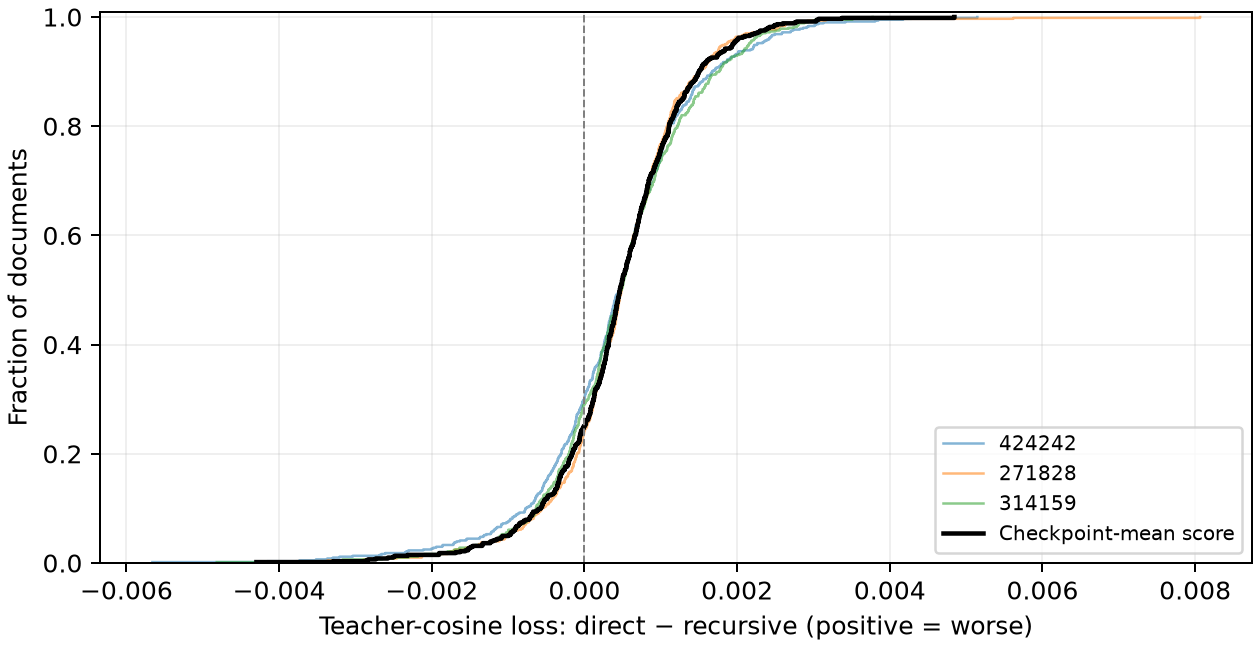
\includegraphics[width=0.96\linewidth]{../results/recursive_reuse_v1/degradation_ecdf.png}
\caption{Empirical distribution of teacher-cosine loss under binary recursive
reuse on the same 606 documents. Positive values indicate degradation relative
to the direct four-child merge. Thin curves show individual checkpoints; the
black curve averages scores within each document before computing the
empirical distribution. This average is not a new ensemble embedding.}
\label{fig:recursive-reuse-loss}
\end{figure}

\subsubsection{Full-Document Execution}
\label{sec:full-results}

The full-document arm recursively processes the complete text of the same 4,000
source documents. Across the population, it represents all \(9{,}142{,}043\)
tokens in \(11{,}356\) contiguous leaves. The longest observed document contains
58,731 tokens and 58 leaves, and the maximum observed recursion depth is 3.
Each seed executes 4,789 internal merges. Dividing the population totals
by 4,000 gives 2,285.51 tokens and 2.839 leaves per document on average.
The maximum-length example is therefore not representative of the typical
evaluated document. The depth histogram is 3,631 documents at depth one,
349 at depth two, and 20 at depth three: only 369 (9.225\%) actually reuse a
generated child in the natural K4 reduction. Only 81 documents (2.025\%) exceed
the backbone's documented 8,192-token context. These counts refer to complete
documents and the original K4 reduction, not the forced binary trees above.
Table~\ref{tab:full-population} reports the per-corpus length summaries;
Table~\ref{tab:full-length-counts} makes the population's length distribution
explicit.

\begin{table}[H]
\caption{Complete-document population, 1,000 documents per corpus. Token
summaries are copied from the frozen official-v6 cache-provenance records,
not from a new model evaluation. Percentiles use the recorded interpolated
values; no pooled percentile is inferred by averaging corpus percentiles.}
\label{tab:full-population}
\centering\small
\begin{tabularx}{\linewidth}{Y r r r r r}
\toprule
\textbf{Corpus} & \textbf{Mean tokens} & \textbf{Median} & \textbf{95th pct.} & \textbf{Max tokens} & \textbf{Max leaves}\\
\midrule
FineWeb-Edu & 2,377.26 & 1,611.5 & 5,886.00 & 58,731 & 58\\
FineWeb & 2,200.02 & 1,504.0 & 5,029.80 & 37,082 & 37\\
OpenWebText & 2,189.23 & 1,574.0 & 5,271.35 & 50,195 & 50\\
Wikipedia & 2,375.53 & 1,749.0 & 5,459.85 & 23,929 & 24\\
\bottomrule
\end{tabularx}
\end{table}

% Generated from verified full-document population metadata.
\begin{table}[H]
\centering\small
\begin{tabularx}{\linewidth}{Yrr}
\toprule
Full-document tokens & Documents & Population (\%) \\
\midrule
1,025--2,048 & 2,707 & 67.675 \\
2,049--4,096 & 924 & 23.100 \\
4,097--8,192 & 288 & 7.200 \\
8,193--16,384 & 61 & 1.525 \\
16,385--32,768 & 15 & 0.375 \\
$>32,768$ & 5 & 0.125 \\
\bottomrule
\end{tabularx}
\caption{Full-document length counts for the original 4,000-document population, not the capped prefixes. Counts exclude special tokens. Global token, leaf and depth histograms are verified against the frozen official results; no new full-root teacher targets are constructed.}
\label{tab:full-length-counts}
\end{table}


\begin{table}[H]
\caption{Unrestricted full-document recursion. Throughput covers recursive
merger and decoder evaluation over cached leaves, including shard loading,
hash and structure validation, device transfers, and telemetry. It excludes
tokenization and teacher leaf embedding and is not a merger-only kernel
benchmark.}
\label{tab:full-document}
\centering
\small
\resizebox{\linewidth}{!}{%
\begin{tabular}{c r c c c c}
\toprule
\textbf{Seed} &
\textbf{Merges} &
\textbf{Child cosine} &
\textbf{Leaf-child cosine} &
\textbf{Recursive-child cosine} &
\textbf{Documents/s} \\
\midrule
424242 & 4,789 & 0.909709 & 0.905621 & 0.968543 & 130.927 \\
271828 & 4,789 & 0.909842 & 0.905757 & 0.968641 & 127.795 \\
314159 & 4,789 & 0.909591 & 0.905485 & 0.968684 & 131.447 \\
\bottomrule
\end{tabular}%
}
\end{table}

Every full root is finite and unique at the tested precision. The pooled and
per-corpus centered numeric rank is 768 for each seed, and no collapse,
geodesic-saturation, or importance-saturation event is observed. The decoder
reconstructs recursive children more closely than original leaf children in
this evaluation, although the protocol does not identify the cause of that
difference.

These full-document measurements assess execution and local behavior; direct
root fidelity is outside this protocol (Section~\ref{sec:evaluation}).

\subsubsection{Local Reconstruction}
\label{sec:retention-results}

Local reconstruction asks how well a decoder can predict the input children
from their parent alone. On the 606 exact-four-child documents, built-in reconstruction is stable across
seeds, and independently fitted parent-only probes exceed their predeclared
fresh-TRAIN floors (Table~\ref{tab:retention}).

\begin{table}[H]
\caption{Official-v6 exact-four-child retention diagnostics. Probes and floors
are fixed using fresh TRAIN data before development and official evaluation.}
\label{tab:retention}
\centering
\small
\resizebox{\linewidth}{!}{%
\begin{tabular}{c c c c c}
\toprule
\textbf{Seed} &
\textbf{Built-in child cosine} &
\textbf{Frozen-probe cosine} &
\textbf{TRAIN floor} &
\textbf{Margin} \\
\midrule
424242 & 0.915040 & 0.908098 & 0.897565 & \(+0.010532\) \\
271828 & 0.915027 & 0.908054 & 0.897558 & \(+0.010497\) \\
314159 & 0.915116 & 0.908151 & 0.897599 & \(+0.010552\) \\
\bottomrule
\end{tabular}%
}
\end{table}

\paragraph{Parent-copy and slot-permutation calibration.}
Predicting the same parent vector in every child slot provides an untrained
control: it tests whether high child cosine requires distinct child predictions.
The matched regenerated comparison in Table~\ref{tab:reconstruction-calibration}
shows only a small built-in decoding gain over learned-parent copy:
\(+0.001043\;[0.001025,0.001060]\), positive on all 606 documents for
checkpoint-mean scores. The released frozen probe instead underperforms copy
by \(0.005916\;[0.005693,0.006151]\), improving only 11 of 606 documents.
Passing the predeclared TRAIN floor therefore does not establish superiority
to this matched, untrained baseline.

% Generated from RESULTS.json; checkpoint scores averaged within documents.
\begin{table}[H]
\caption{Matched reconstruction calibration on 606 four-child prefixes. Learned rows average checkpoint scores, not vectors. Copy rows repeat one unit parent in all four output slots. $\Delta$ compares each row with learned-parent copy; only the decoder/probe rows isolate a decoding gain for that same parent. Shuffled scoring averages all 24 within-document target permutations, holding inputs and predictions fixed. Order gap is ordered minus shuffled cosine.}
\label{tab:reconstruction-calibration}
\centering\small
\begin{tabularx}{\linewidth}{Yrrrr}
\toprule
Prediction rule & Child cosine & $\Delta$ vs copy & Shuffled & Order gap \\
\midrule
Learned parent copied & 0.914022 & +0.000000 & 0.914022 & +0.00000000 \\
Built-in strict decoder & 0.915064 & +0.001043 & 0.915063 & +0.00000069 \\
Released TRAIN-fitted probe & 0.908105 & -0.005916 & 0.907197 & +0.00090843 \\
Weighted pooling copied & 0.920365 & +0.006344 & 0.920365 & +0.00000000 \\
Unweighted pooling copied & 0.922576 & +0.008554 & 0.922576 & +0.00000000 \\
\bottomrule
\end{tabularx}
\end{table}


Copying either pooling parent outperforms both learned decoding rules
(Table~\ref{tab:reconstruction-calibration}). The built-in decoder trails
weighted and unweighted copy by \(0.005301\) and \(0.007511\), respectively,
on every document after averaging checkpoint scores. These are untrained copy
baselines, not the fitted pooling probes below: high child cosine is attainable
without distinct child predictions or recovered order.

The order gap compares correct slot assignments with the mean over all target
permutations. The built-in decoder's order gap is just \(6.8555\times10^{-7}\), with paired
95\% interval \([5.9645,7.7248]\times10^{-7}\): its mean cosine is almost
unchanged by target-slot permutation. The frozen probe has a larger order gap,
\(0.000908\;[0.000699,0.001116]\), despite its lower overall reconstruction
score. Thus order sensitivity and average reconstruction quality need not move
together. The corresponding nine-derangement gaps are \(9.1407\times10^{-7}\)
and \(0.001211\), while every copy baseline has exactly zero gap up to numerical
precision. Even the probe's oracle best-assignment mean, \(0.911371\), remains
below learned-parent copy. These diagnostics do not demonstrate losslessness
or robust recovery of document-specific order.

\begin{figure}[H]
\centering
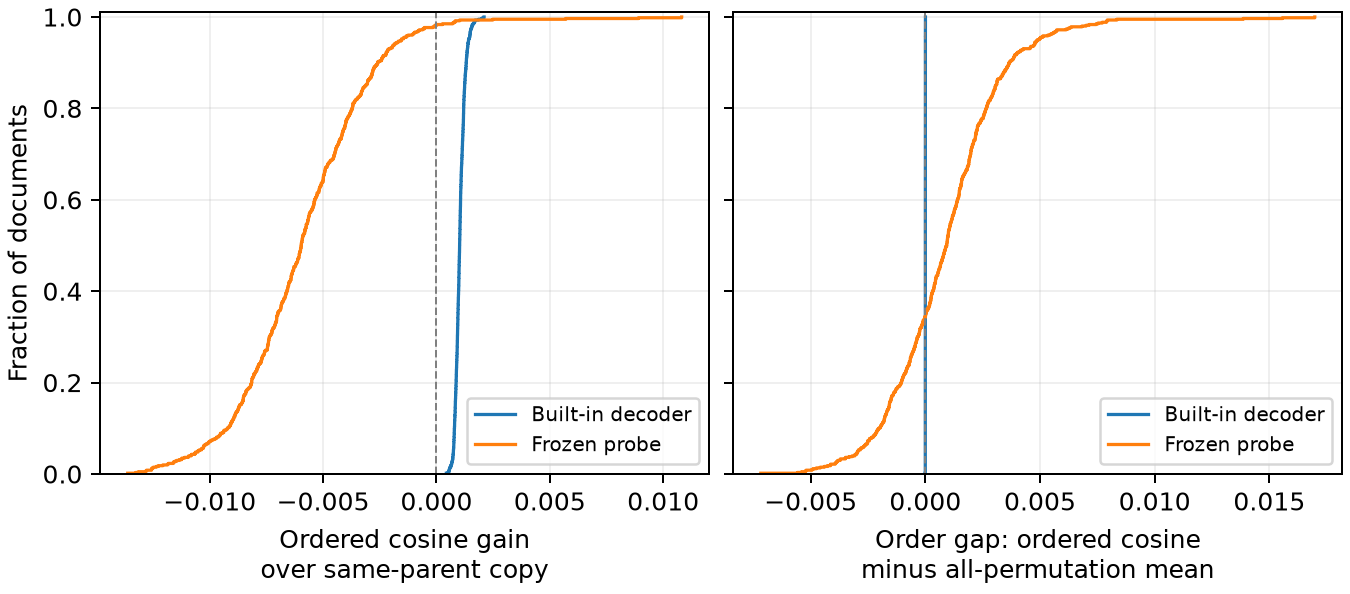
\includegraphics[width=\linewidth]{../results/reconstruction_calibration_v1/calibration_ecdf.png}
\caption{Per-document reconstruction calibration, averaging checkpoint scores
within each document. Left: ordered-cosine gain over copying the same learned
parent. Right: ordered minus mean shuffled-target cosine. Positive values favor
the decoder or the original slot assignment, respectively. The built-in
order-gap curve lies near zero at the probe's scale; its small nonzero mean
is reported in the text.}
\label{fig:reconstruction-calibration}
\end{figure}

\paragraph{Matched K4 comparison with fitted pooling probes.}
The single-checkpoint matched experiment evaluates the frozen seed-424242 clean-v6 checkpoint
on the same 606 exact-K4 official documents. Table~\ref{tab:k4-pooling} reports
the parent-only probe results and paired document-level bootstrap intervals.

\begin{table}[H]
\caption{Matched exact-K4 parent-only probe comparison on 606 official
documents. Difference columns are paired document-level differences; negative
values favor pooling. The experiment uses the frozen seed-424242 clean-v6
checkpoint.}
\label{tab:k4-pooling}
\centering
\small
\begin{tabularx}{\linewidth}{Y C C C}
\toprule
\textbf{Parent representation} &
\textbf{Mean child cosine} &
\textbf{Learned minus baseline} &
\textbf{95\% CI} \\
\midrule
Learned clean-v6 parent & \(0.908105\) & -- & -- \\
Token-weighted normalized mean &
\(0.910180\) &
\(-0.002075\) &
\([-0.002227,-0.001935]\) \\
Unweighted normalized mean &
\(0.912320\) &
\(-0.004215\) &
\([-0.004710,-0.003749]\) \\
\bottomrule
\end{tabularx}
\end{table}


Both paired confidence intervals favor pooling under the evaluated residual
probe. Decoder-dependence and recovery limits are discussed in
Section~\ref{sec:limitations}.

In the full-document arm, the built-in decoder is evaluated at every one of the
4,789 merges per seed and maintains overall child cosine between \(0.909591\)
and \(0.909842\). These values describe local reconstruction under the built-in decoder;
the frozen-probe comparison is a separate safe-arm measurement. The matched pooling comparison applies only to the
safe exact-K4 subset and does not provide a full-document pooling reference.

\subsubsection{Changes During the Final Training Stage}
\label{sec:continuation-results}

To distinguish inherited performance from changes in the final training stage,
we compare each initialization-source merger with its final checkpoint.
The matched source--final comparison shows that continuation barely changes
teacher fidelity: 99.96\% of the final gain over weighted pooling is already
present in the inherited source mergers. Source and final teacher cosines round
to the same six-decimal value in Table~\ref{tab:continuation-comparison}; their
parents have cosine \(0.999999912\). The small positive teacher-cosine change
occurs on 2,263/4,000 documents (56.6\%) after averaging checkpoint scores.

% Generated from fixed RESULTS.json; document-paired intervals.
\begin{table}[H]
\centering\footnotesize
\begin{tabularx}{\linewidth}{Yrrr}
\toprule
Metric (documents) & Source & Final & Change [95\% CI] $(\times10^{-6})$ \\
\midrule
Teacher cosine (4,000) & 0.985045 & 0.985045 & +0.847 [+0.610, +1.081] \\
Source AUC (2,000 held out) & 0.584827 & 0.584294 & -533.292 [-675.928, -392.327] \\
Parent-copy cosine (606) & 0.914069 & 0.914022 & -47.389 [-48.109, -46.613] \\
Probe cosine (606) & 0.908114 & 0.908105 & -9.416 [-11.671, -7.102] \\
Probe gain over copy (606) & -0.005954 & -0.005916 & +37.973 [+35.859, +40.216] \\
Probe order gap (606) & 0.000910 & 0.000908 & -1.872 [-3.767, +0.202] \\
\bottomrule
\end{tabularx}
\caption{Matched continuation comparison on regenerated safe prefixes. Teacher cosine uses all 4,000 documents; pooled source AUC uses the same 2,000 held-out document pairs at each stage. Reconstruction uses the same 606 exact-four prefixes and each stage's separately fitted, released TRAIN probe. Gain subtracts copying that stage's own parent; order gap subtracts the mean over all 24 target assignments. Lower AUC is preferred; higher cosine/gain is preferred. Intervals condition on the fixed checkpoints, probes and selected classifiers. Changes and interval bounds are in units of $10^{-6}$; source/final columns are unscaled.}
\label{tab:continuation-comparison}
\end{table}


Source-detection AUC falls slightly at the pooled level for all three
checkpoints. Logistic regression remains the strongest observed family at both
endpoints in every scope; both attack families are retained. Changes are not
uniform across strata: Wikipedia AUC rises by \(0.000100\), with interval
\([-0.000209,0.000409]\), while teacher cosine falls slightly for Wikipedia
and three-child prefixes, with intervals spanning zero.

On the 606 exact-four prefixes, absolute probe cosine decreases, but
parent-copy cosine decreases more. The probe's copy-relative gain therefore
becomes less negative on 559/606 documents (92.2\%), without either probe
outperforming copy. The order-gap change also fails to establish greater order
recovery. Table~\ref{tab:continuation-comparison} gives the paired estimates and
intervals; Figure~\ref{fig:continuation-comparison} shows document-level changes.

\begin{figure}[H]
\centering
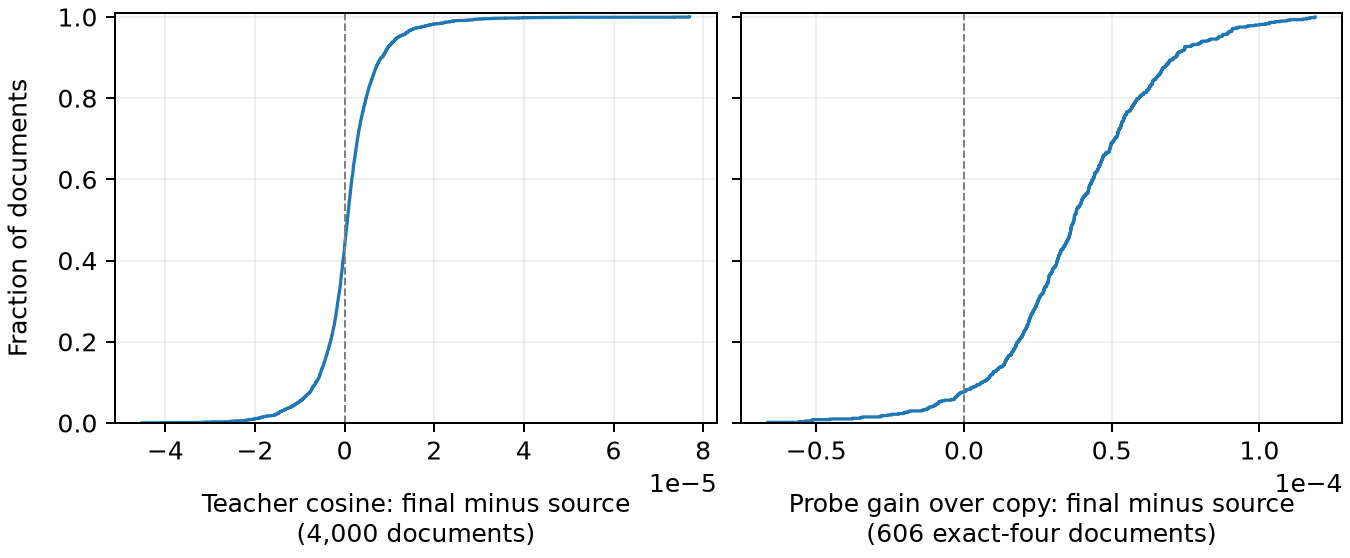
\includegraphics[width=\linewidth]{../results/continuation_comparison_v1/continuation_ecdf.png}
\caption{Checkpoint-mean document changes between matched source and final
endpoints. Left: teacher cosine on 4,000 prefixes. Right: probe gain over
copying each stage's own parent on 606 exact-four prefixes. Positive values
favor the final endpoint on the indicated contrast; the right panel does not
imply a positive decoding gain or higher absolute probe cosine.}
\label{fig:continuation-comparison}
\end{figure}

The inherited mergers therefore account for almost all measured advantage over
pooling. Interpretation of the bundled continuation and its training history
is discussed in Section~\ref{sec:limitations}.

\subsubsection{Order, Trees, and Segmentation}
\label{sec:extended-structure-results}

Recomputing parents after input permutation tests whether decoder outputs
follow the reordered children; permuting only scoring assignments provides
a negative control with the parent fixed. On 606
four-leaf documents, the released built-in decoder's original-order gap is
\(6.86\times10^{-7}\) but its mean following gap (matched-minus-shuffled child cosine after
recomputing the parent for each input permutation) across all 24 actual-mass
input permutations is \(-3.12\times10^{-9}\) (95\% interval
\([-3.23,-3.02]\times10^{-9}\)). For the released candidate probe, the
respective gaps are \(0.000908\) and \(-0.00000418\) (interval
\([-0.00000474,-0.00000364]\)). Equal-mass controls give similar signs;
fixed-parent scoring-only means vanish to numerical precision. These are
\emph{target-child} assignment comparisons, not proof about teacher embeddings
of permuted text or absolute information content.

Each of the five ordered binary trees loses teacher cosine relative to the
direct four-leaf merge: checkpoint-mean deltas range from \(-0.000461\) to
\(-0.000678\), all with document-paired intervals below zero. Grouping choice
matters slightly even when leaf count and binary arity are fixed. In contrast,
resegmenting the same text into 512-token K4 leaves loses \(0.010060\)
teacher cosine versus original 1,024-token K4 leaves; 256-token K4 loses
\(0.022253\). With matched within-segmentation weighted pools as references,
K4 retains advantages of \(0.012912\) and \(0.024322\), respectively;
the reference itself changes along with the leaves. These losses combine
leaf granularity, number of merges, distribution shift, and depth, and do not
measure a pure tree effect or support arbitrarily fine splitting.

\subsubsection{Probe and Gradient-Path Controls}
\label{sec:extended-probe-results}

To test whether reconstruction comparisons depend on the chosen decoder,
matched TRAIN-only fits compare three probe families. Across three checkpoints
and three probe seeds, learned-parent ordered child cosine is \(0.912004\)
for the bounded residual, \(0.908634\) for the unbounded residual, and
\(0.764288\) for the direct non-residual MLP. Learned minus weighted-pool
probe cosine changes sign across these families: \(-0.002026\), \(+0.000523\),
and \(-0.000684\), respectively. The corresponding learned-probe gains over
copying the learned parent are \(-0.002017\), \(-0.005387\), and
\(-0.149733\); these TRAIN fits therefore do not establish superior local
reconstruction. Poor performance of the direct MLP may reflect its architecture
or fit, not an information-theoretic limit. These fits are separate from the
unavailable matched-pooling probes.

The gradient-path intervention compares joint training with reconstruction
gradients allowed to reach the merger (attached) or blocked at the decoder
input (detached). Under this intervention, attached minus detached teacher
cosine is \(-1.5653\times10^{-6}\) (document-paired 95\% interval
\([-1.9905,-1.1424]\times10^{-6}\)); source-detection AUC changes by
\(-0.000427\) (interval \([-0.000755,-0.000109]\)), with a lower AUC indicating
less detectable model vectors. Raw ordered reconstruction changes by
\(-0.00008362\); parent-copy cosine also falls, yielding a \emph{positive}
copy-relative gain contrast of \(+0.00000555\). This controlled contrast
has mixed directions and extremely small magnitudes, and cannot attribute
the historical source--final endpoints to the decoder objective. Fixed
classifier families and fixed training seeds limit the intervals.

\subsection{Downstream Utility: Long-Document Retrieval}
\label{sec:retrieval-results}
Teacher agreement need not imply useful document rankings. We therefore
evaluate retrieval with frozen queries and document representations on four
LongEmbed tasks. Table~\ref{tab:review-retrieval} compares the first leaf,
full-document pooling, and recursive composition with direct teacher-prefix
references. Mean-prefix uses masked-mean hidden states; CLS-prefix uses the
backbone's first-token representation.
\begin{table}[t]
\caption{Complete frozen LongEmbed task corpora; query-weighted nDCG@10
(higher is better). Recursive scores average the three fixed model scores
\emph{per query}, not their document vectors. Mean-pool queries match all
mean-based rows; CLS queries match only CLS-prefix documents. Prefix teacher
references truncate at the teacher context; the weighted, unweighted, and
recursive documents use all chunks. Different query interfaces make the CLS
reference a useful comparator, not a controlled pooling ablation.}
\label{tab:review-retrieval}
\centering\small
\begin{tabular}{lrrrrrr}
\toprule
Task & First & Weighted & Unweighted & Mean-prefix & CLS-prefix & Recursive \\
\midrule
2WikiMQA & 0.2044 & 0.2643 & 0.2752 & 0.2776 & 0.8709 & 0.2768 \\
QMSum & 0.1996 & 0.2590 & 0.2533 & 0.2524 & 0.4069 & 0.2390 \\
SummScreenFD & 0.5541 & 0.7998 & 0.7933 & 0.6942 & 0.9314 & 0.7728 \\
NarrativeQA & 0.0449 & 0.0835 & 0.0830 & 0.0620 & 0.3015 & 0.0790 \\
\bottomrule
\end{tabular}
\end{table}

Against the full-document weighted pool, recursive nDCG@10 changes by:
\begin{itemize}[nosep,leftmargin=2em]
\item 2WikiMQA: \(+0.01250\), positive-document-cluster 95\% interval
  \([+0.00253,+0.02268]\);
\item QMSum: \(-0.01995\), interval \([-0.02982,-0.01007]\);
\item SummScreenFD: \(-0.02700\), interval \([-0.03893,-0.01479]\);
\item NarrativeQA: \(-0.00448\), interval \([-0.00854,-0.00010]\).
\end{itemize}
Higher short-prefix teacher agreement did not translate into a consistent
retrieval advantage over simple pooling.
The CLS-reference advantage on every task makes the documented-interface
mismatch consequential; it does not show that changing only the aggregation
method would reproduce CLS performance. In the 355-document, 10,449-query
NarrativeQA task, 347 documents exceed 8,192 tokens, 85 exceed the configured
96-leaf training cap, the maximum has 477 leaves, and K4 depth reaches five.
These roots are computed and ranked but lack direct untruncated teacher targets.
Bootstrap components number 300, 197, 336, and 355 across the four tasks;
all fixed candidate sets and all task outcomes are retained, including
length-stratified and secondary metrics in the result JSON.

\subsection{Supporting Architecture and Scaling Studies}
\label{sec:architecture-scaling}

To examine the trade-off between fewer reduction levels and larger merges,
a matched validation-only scaling study compares binary, four-way, and
eight-way systems on the same eight-child (K8) cache. The evaluated systems differ in
parameter count and training history, so Table~\ref{tab:arity} is a
system-level comparison rather than a causal estimate of arity alone.

\begin{table}[H]
\caption{Matched validation-only arity comparison. Throughput and depth are
specific to this scaling protocol and are not directly comparable with the
official full-document throughput in Table~\ref{tab:full-document}.}
\label{tab:arity}
\centering
\small
\resizebox{\linewidth}{!}{%
\begin{tabular}{l r c c c c}
\toprule
\textbf{Configuration} &
\textbf{Parameters} &
\textbf{Strongest \(A_{\mathrm{safe}}\)} &
\textbf{Teacher cosine} &
\textbf{Mean/max depth} &
\textbf{Documents/s} \\
\midrule
Binary (\(K=2\)) & 73.1M & 0.647113 & 0.977828 & 1.597 / 4 & 4,811.13 \\
Four-way (\(K=4\)) & 111.5M & 0.592991 & 0.978854 & 1.140 / 2 & 5,256.61 \\
Eight-way (\(K=8\)) & 124.1M & 0.668336 & 0.977910 & 1.024 / 2 & 5,255.50 \\
\bottomrule
\end{tabular}%
}
\end{table}


In Table~\ref{tab:arity}, relative to the binary reference, the evaluated K4 system reduces mean depth by
28.6\% on this panel and increases measured throughput while improving both
cosine and detectability. Moving from K4 to K8 reduces mean depth by a further
10.2\% but provides essentially no throughput gain, worsens detectability, and
reaches 12.5\% batch saturation at training step 581. Among these evaluated
systems, K4 provides the strongest overall trade-off under the protocol; the
comparison does not show that arity alone caused the differences.

Two additional controls did not improve the selected system. A K4 model using
approximately 510-token leaves obtained macro cosine \(0.97143\) and FineWeb
cosine \(0.96828\), failing its configured cosine guard. A wider K4 model with
hidden width 1,152 and 166.9 million parameters reached validation2 AUC
\(0.62058\) and exhibited training saturation.

\section{Discussion}
\label{sec:discussion}

The experiments separate recursive executability from teacher fidelity and
downstream utility.

\subsection{Teacher Fidelity at a Higher Composition Cost}

Learning improves agreement with the masked-mean teacher, but the small gain
comes at a substantial composition cost. This makes the choice between pooling
and learned composition an application-level trade-off, not a general ranking
of representation methods. A system that specifically values agreement with
this teacher may accept the extra cost; a system that needs inexpensive document
vectors has no consistent retrieval evidence here for replacing pooling.

Paired cosine and marginal detectability answer different questions. Permuting
teacher vectors across documents would preserve their marginal distribution
while destroying document-to-vector assignments. Meeting the predeclared
pooled detection criterion therefore does not establish distributional equality,
and neither diagnostic substitutes for downstream evaluation. The strong
retrieval reference based on the encoder's CLS token, rather than a mean of
token states, shows why the pooling interface also needs evaluation. Because
that reference differs in both interface and truncation, it does not isolate
the effect of either choice.

The source checkpoints already contain almost all of the final fidelity
advantage over pooling. The matched continuation comparison consequently
supports little additional benefit from the final training stage, rather than
an explanation of how the original advantage arose. Comparing the merger's weighted spherical reference with its corrected output
shows that the correction helps this trained system;
attribution to geometry or individual objectives requires the controlled
comparisons described in Section~\ref{sec:limitations}.

\subsection{Recursive Execution and Local Reconstruction}

Full-document runs bridge the gap between a prefix-only fidelity test and
execution on longer inputs: the shared merger produces finite roots beyond
the teacher's direct context. Tree and segmentation interventions nevertheless
show that the ability to reuse an output does not make the result independent
of how the text is divided and merged. The tested resegmentations produce
larger fidelity losses than the tested regroupings, but they change leaf
representations and depth together.
Successful execution alone cannot establish the quality of deeper roots.

Local reconstruction is also a weaker property than recovering a document
from its final root. The decoder receives each intermediate parent separately, not just the final
document vector. Predicting the same parent vector for every child already
explains much of the absolute reconstruction score. The decoder's limited ability to distinguish child positions and the stronger
baselines that copy a pooled vector into every position caution against interpreting
high child cosine as recovery of distinct ordered constituents. These results
support local predictability, not losslessness or preserved mutual information.

\subsection{Limitations and Future Work}
\label{sec:limitations}

\paragraph{Representation and task scope.}
The evidence is specific to one teacher interface and a narrow set of English tasks.
All fitting and teacher-fidelity tests use one 768-dimensional masked-mean
teacher and four English corpora. The separately pinned retrieval benchmark
covers four English tasks, not classification or clustering, and the strong
CLS reference shows that the representation interface matters.

\textbf{Proposed remedy.} Train a merger on CLS-based representations with
consistent chunk, query, and document interfaces. Compare encoders and languages
on independently sourced retrieval, classification, and clustering tasks to
test whether improved teacher fidelity translates into broader utility.

\paragraph{Population and recursive scale.}
The evaluated population does not establish fidelity at unrestricted recursive depth.
Selecting the first 1,000 length-eligible documents per corpus is not random
sampling. The full arm mostly contains short documents: only 81 exceed the
backbone context and only 20 reach natural K4 depth three. LongEmbed reaches
K4 depth five, but supplies rankings rather than direct untruncated-root
teacher targets. The five-tree and two-finer-chunk tests still couple leaf
representations, arity, and depth. Development and official populations are disjoint, so their difference is not
a paired improvement estimate.

\textbf{Proposed remedy.} Use length-stratified populations extending beyond
the configured 96-leaf training cap, and vary segmentation, arity, and depth
separately. Direct fidelity tests of deeper roots require a longer-context
teacher or another evaluation design. Audit exact and near duplicates across
corpora and continuation-training data. Comparisons matched on prefix length,
arity, and content would help explain domain-specific detectability.

\paragraph{Training and causal comparisons.}
The available comparisons do not isolate the causes of the fidelity gain.
Clean-v6 starts from trained source mergers; its final 400 updates describe
neither from-scratch training nor complete training cost. Matched source/final
endpoints cannot isolate one component of the continuation bundle. The
attached/detached intervention has small, mixed outcomes: it changes one
gradient route in a small exact-four TRAIN regime, starting from trained source
encoders, rather than removing the decoder loss from the full training recipe.
Arity comparisons also differ in capacity and training history.

\textbf{Proposed remedy.} Train from-scratch, matched-budget lineages with
true decoder-loss removal and matched geometry and arity alternatives. These
comparisons would help isolate which objectives and architectural choices
contribute to the fidelity gain.

\paragraph{Reconstruction and geometry.}
The reconstruction evidence depends on decoder capacity, fitting, and geometric constraints.
The bounded residual decoder restricts output directions
(Section~\ref{sec:strict-decoder}); unit norm and bounded geodesic movement do
not guarantee a teacher-distribution manifold or semantic preservation. The
local results above do not rule out recovery by other decoders. The matched
pooling reconstruction study covers one final checkpoint and one residual
probe family. Fixed-budget bounded, unbounded, and direct probes are separate
TRAIN-fitted models, with varying family rankings and direct-model fit;
unconstrained outputs remove a structural restriction, not optimization or
data dependence. The missing matched-pooling probe binaries also prevent exact
copy/permutation calibration of those fits.

\textbf{Proposed remedy.} Retain matched probes across representations,
seeds, and fitting budgets, and check their optimization. Test recovery from
the final document root, not only intermediate parents, using both input-order
and target-slot controls to distinguish recovery of ordered constituents from
prediction of shared content.

\paragraph{Statistical and confirmatory scope.}
The reported intervals are conditional diagnostics, not independent confirmation of broad claims.
The study evaluates three final checkpoints, one attack split, and two
classifier families. The uncertainty protocol in
Section~\ref{sec:detectability} conditions on fixed models, inputs, and selected
attacks rather than the full training and selection process. Task-specific
retrieval intervals are not a cross-task meta-analysis; the AUC criterion is
not an equivalence or privacy guarantee, and TRAIN-derived probe floors are
not matched-population noninferiority tests.
The safe-arm baseline, recursive-reuse, reconstruction-calibration, tree/order,
and continuation comparisons reuse evaluated documents and regenerated inputs.
LongEmbed uses a distinct population, but its system and hypotheses were fixed
after the initial evaluation.

\textbf{Proposed remedy.} Preregister evaluations on fresh documents with
more training seeds, attack splits, refitted attackers, and independent tasks.
These comparisons would assess robustness beyond the current conditional
estimates and separate exploratory findings from confirmatory evidence.

\paragraph{Cost and reproducibility.}
Composition timings do not measure end-to-end value, and reproduction has documented discrepancies.
The fidelity--cost comparison measures composition only on the identified
GPU. Cached-leaf pipeline throughput measures a different workload; neither
measures end-to-end embedding cost. 
Artifact identities, regenerated-cache constraints, numerical repairs, and
reproduction discrepancies are documented in
Appendices~\ref{app:safe-baseline-reproduction}
and~\ref{app:reconstruction-calibration} and the associated audit subsections.

\textbf{Proposed remedy.} Benchmark text encoding, composition, storage,
and inference together. Independently reproduce the results using the pinned
inputs, retained artifacts, and documented numerical protocol to assess the
discrepancies and the quality--cost trade-off in a complete application.

\section{Conclusion}
\label{sec:conclusion}

The central idea is to merge embeddings into another embedding that can be
merged again, without leaving the frozen encoder's output coordinates,
embedding dimension, or unit-sphere domain. The shared geodesic merger provides
that reusable interface; teacher supervision seeks to align each parent with
the encoder's representation of its combined text. Structural reusability is
provided by the construction, while semantic fidelity remains empirical.

The evaluated system improves short-prefix teacher fidelity over pooling at
substantial composition cost, but recursive results depend on segmentation
and merge structure, and reconstruction and retrieval show no consistent
advantage. Pooling remains a simple, inexpensive comparator. The evidence
therefore supports the feasibility of
learned, recursively reusable embeddings in the original geometric domain,
not guaranteed semantic preservation or a general downstream advantage.

\bibliographystyle{tmlr}
\bibliography{references}
\clearpage

\appendix

The appendices provide the full training recipe
(Appendix~\ref{app:training-objectives}), artifact identities and experimental
reproduction details (Appendix~\ref{app:reproducibility}), and analytical
bounds, parameter counts, and timing definitions (Appendix~\ref{app:geometry}).

\section{Complete Training Objectives and Optimization Schedule}
\label{app:training-objectives}

This appendix gives the complete definitions and coefficients summarized in
Section~\ref{sec:training-objectives}.
The goal of training is to make each generated parent embedding match the frozen teacher where a valid direct teacher target exists, while also keeping the distribution of generated embeddings close to the teacher distribution and preserving recoverable information about the child representations. Let \(z\) denote a generated parent embedding and \(t\) the normalized direct teacher embedding of the corresponding combined text span. The primary supervision is cosine distance,

\[
\mathcal{L}_{\mathrm{teacher}}
=
1-\operatorname{cos}(z,t).
\]

Minimizing this loss encourages the generated parent to align with its corresponding teacher representation in the teacher embedding space. A direct teacher target is available only when the complete represented span lies within the safe range for direct teacher encoding. If a recursive node represents a span beyond this range, no full-span teacher target is constructed, and that node contributes no teacher-cosine term.

Paired cosine similarity constrains each generated embedding relative to its own teacher target, but it does not by itself constrain systematic differences between the generated and teacher embedding distributions. We therefore additionally match minibatch-level first and diagonal second moments. For the \(M\) generated--teacher pairs in a minibatch that have valid direct targets, let \(\mu_z\) and \(\mu_t\) denote the corresponding mean vectors, and let \(\sigma_z^2\) and \(\sigma_t^2\) denote their coordinate-wise variance vectors. The distribution losses are

\[
\mathcal{L}_{\mathrm{mean}}
=
\lVert \mu_z-\mu_t\rVert_2^2,
\qquad
\mathcal{L}_{\mathrm{var}}
=
\lVert \sigma_z^2-\sigma_t^2\rVert_2^2.
\]

The variance uses the population denominator \(M\), independently for each
embedding dimension, rather than a full covariance matrix. The vectors are
collected across all teacher-supervised merges in the optimizer minibatch. These terms are applied when at least eight matched generated--teacher pairs are available in the minibatch, with coefficients

\[
\lambda_{\mathrm{mean}}=0.25,
\qquad
\lambda_{\mathrm{var}}=256.
\]

The learned semantic composition weights are also regularized relative to the structural token-mass prior. Recall that \(q_i\) is the relative token mass, \(w_i\) is the learned semantic composition weight, and \(\delta_i\) is the learned salience correction. The prior regularizer is the Kullback--Leibler divergence \cite{kullback-leibler-1951-information},

\[
\mathcal{L}_{\mathrm{prior}}
=
D_{\mathrm{KL}}(q\,\|\,w)
=
\sum_{i=1}^{k}q_i\bigl(\log q_i-\log w_i\bigr),
\]

which discourages unnecessary departures from the structural token-mass prior without forcing \(w_i=q_i\). The magnitude of the salience corrections is regularized by

\[
\mathcal{L}_{\delta}
=
\frac{1}{N_{\mathrm{active}}}
\sum_{\text{active }i}\delta_i^2,
\]

where \(N_{\mathrm{active}}\) is the number of active child slots included in the average.

To discourage the learned weights from becoming excessively concentrated relative to the token-mass prior, define

\[
H(p)=-\sum_i p_i\log p_i
\]

and use the sharpness penalty

\[
\mathcal{L}_{\mathrm{sharp}}
=
\left[
\max\!\left(H(q)-H(w)-0.1,\,0\right)
\right]^2.
\]

Finally, slot-use regularization discourages a persistent preference for a particular ordered merger position that is not explained by structural token mass:

\[
\mathcal{L}_{\mathrm{slot}}
=
\sum_{j=1}^{4}
\left(
\mathbb{E}_{\mathrm{batch}}[w_j]
-
\mathbb{E}_{\mathrm{batch}}[q_j]
\right)^2.
\]

The four semantic-salience regularizers use equal coefficients,

\[
\lambda_{\mathrm{prior}}
=
\lambda_{\delta}
=
\lambda_{\mathrm{sharp}}
=
\lambda_{\mathrm{slot}}
=
0.01.
\]

At full strength, the merger-only objective is therefore

\[
\begin{aligned}
\mathcal{L}_{\mathrm{enc}}
={}&
\mathcal{L}_{\mathrm{teacher}}
+0.25\mathcal{L}_{\mathrm{mean}}
+256\mathcal{L}_{\mathrm{var}}\\
&+0.01\mathcal{L}_{\mathrm{prior}}
+0.01\mathcal{L}_{\delta}
+0.01\mathcal{L}_{\mathrm{sharp}}
+0.01\mathcal{L}_{\mathrm{slot}}.
\end{aligned}
\]

The teacher term encourages paired agreement with the teacher, the mean and variance terms provide minibatch-level distribution matching, and the salience regularizers constrain semantic reweighting while preserving the distinction between learned importance and exact token mass.

The autoencoder variant adds a strict training-time decoder \(D_\phi\) that receives only the generated parent embedding \(z\). From this parent, it predicts four ordered child embeddings \(\hat{x}_1,\ldots,\hat{x}_4\) and importance logits that are normalized to predicted importance weights \(\hat{w}_1,\ldots,\hat{w}_4\). The decoder is not given the true child embeddings, child token counts, token-mass fractions \(q_i\), encoder salience corrections, encoder semantic weights as inputs, corpus or source identity, or reduction-tree metadata.

For genuine four-child training merges, ordered child reconstruction is trained with

\[
\mathcal{L}_{\mathrm{recon}}
=
1-\frac{1}{4}
\sum_{i=1}^{4}
\operatorname{cos}(\hat{x}_i,\operatorname{sg}(x_i)),
\]

where \(\operatorname{sg}\) denotes stop-gradient. Each decoder output slot
is compared with the corresponding ordered input child; recursively generated
children are detached on this target branch. The reconstruction coefficient is

\[
\lambda_{\mathrm{recon}}=0.15.
\]

The decoder also predicts the semantic importance distribution used by the merger. With the encoder's learned effective weights \(w\) detached from the decoder target, the importance loss is

\[
\mathcal{L}_{\mathrm{imp}}
=
D_{\mathrm{KL}}(w\,\|\,\hat{w})
=
\sum_{i=1}^{4}
w_i\bigl(\log w_i-\log \hat{w}_i\bigr),
\]

with coefficient

\[
\lambda_{\mathrm{imp}}=0.025.
\]

A cycle-consistency term additionally recomposes the predicted children using the decoder-predicted importance weights,

\[
\hat{z}
=
\operatorname{normalize}\!\left(
\sum_{i=1}^{4}\hat{w}_i\hat{x}_i
\right),
\]

and compares this spherical recomposition with the original parent:

\[
\mathcal{L}_{\mathrm{cycle}}
=
1-\operatorname{cos}(\hat{z},\operatorname{sg}(z)),
\qquad
\lambda_{\mathrm{cycle}}=5.0.
\]

This cycle uses the weighted spherical reference construction rather than
another complete Transformer merge. The reference parent is detached, while
the parent supplied to the decoder remains differentiable during joint
training. During decoder-only fitting that decoder input is detached too. A low cycle loss alone does not establish recovery of the original children, since the encoder and decoder could become mutually consistent without accurately reconstructing their inputs; direct ordered-child reconstruction is therefore treated separately.

At full strength, the autoencoder objective can be written compactly as

\[
\mathcal{L}_{\mathrm{AE}}
=
\mathcal{L}_{\mathrm{enc}}
+0.15\mathcal{L}_{\mathrm{recon}}
+5.0\mathcal{L}_{\mathrm{cycle}}
+0.025\mathcal{L}_{\mathrm{imp}}.
\]

Optimization is staged. During the first 300 updates, the merger is frozen and the strict decoder is trained on full-arity examples using the reconstruction and importance objectives. The merger is then unfrozen for 100 joint encoder--decoder updates. For joint update \(s\in\{301,\ldots,400\}\), define

\[
\gamma_s=\frac{s-300}{100}.
\]

The teacher and distribution-matching terms are applied at their full coefficients during joint training, while the semantic regularizers, reconstruction loss, cycle loss, and importance loss are multiplied by \(\gamma_s\). Thus, the joint objective is

\[
\begin{aligned}
\mathcal{L}_{\mathrm{joint}}(s)
={}&
\mathcal{L}_{\mathrm{teacher}}
+0.25\mathcal{L}_{\mathrm{mean}}
+256\mathcal{L}_{\mathrm{var}}\\
&+\gamma_s\Bigl(
0.01\mathcal{L}_{\mathrm{prior}}
+0.01\mathcal{L}_{\delta}
+0.01\mathcal{L}_{\mathrm{sharp}}
+0.01\mathcal{L}_{\mathrm{slot}}\\
&\hspace{2.8em}
+0.15\mathcal{L}_{\mathrm{recon}}
+5.0\mathcal{L}_{\mathrm{cycle}}
+0.025\mathcal{L}_{\mathrm{imp}}
\Bigr).
\end{aligned}
\]

The frozen teacher supplies training supervision, while the strict decoder provides auxiliary reconstruction objectives and can also be invoked for retention diagnostics. Recursive document representations themselves are produced by the merger, so normal recursive inference does not require either a direct teacher target or the decoder.

\subsection{Recursive Loss Reduction and Gradient Flow}
\label{app:loss-reduction}

In the contiguous K4 path, sampled rows are grouped by leaf count for batched
execution. Every reduction level is executed, carrying singleton remainders.
Within a leaf-count group, teacher cosine is averaged over valid parent--target
pairs at each level and then equally over levels that have teacher targets.
Reconstruction and cycle losses are averaged over genuine four-child merges
within each level, then over reduction levels; a level with no genuine
four-child merge contributes zero to those terms. Group-level supervised
losses are weighted by the number of rows in the group when forming the
minibatch objective. Consequently, this is not a uniform average over all
internal nodes in the minibatch.

Moment matching instead pools every valid generated--teacher pair across the
whole minibatch, uses population coordinate variances, and is disabled when
fewer than eight pairs are available. Salience regularizers are computed at
each batched merge call and averaged over the collected calls; importance
losses are averaged over decoder calls with genuine four-child targets.
Inactive salience slots carry zero mass. These implementation-level reduction
choices define the scale of the stated loss coefficients.

Cached leaf vectors and teacher targets are fixed. Generated parents remain
connected through subsequent merger calls during joint optimization, so
teacher-supervised ancestors can supply gradients through earlier merges.
Child reconstruction targets, importance targets, and the reference side of
the cycle loss are detached as specified above. The notation for an individual
node does not imply a different, uniformly node-weighted training objective.

\section{Reproducibility and Additional Experimental Details}
\label{app:reproducibility}

This appendix identifies the models and data needed to reproduce the reported
evaluations. Shared release, classifier, and dataset settings come first;
study-specific subsections then describe input regeneration, checks, and
recorded recoveries. File names retain the experiment labels used in the
repository.

\subsection{Checkpoint Lineage and Release Availability}
\label{app:lineage}

The final models continue from released source autoencoders. Merger parameters
are loaded; decoder parameters are discarded and reinitialized; the final
checkpoint is fixed at continuation step 400 before development access.
The published identities below define that continuation exactly. They do not
specify a complete from-scratch training history for the source mergers.
Available reproduction materials identify the released weights, architecture,
and source-to-final continuation; they do not establish the complete
source-training schedule or total training budget.

The terms \emph{clean-v6} and
\emph{official-v6} identify the final training/evaluation protocol and its final
evaluation, respectively; \texttt{v1-paper} is a publication-release label, not
an earlier trained model. In particular, the
checkpoint called ``V1'' in the matched-pooling artifacts is the final
clean-v6 seed-424242 checkpoint, identified by the same SHA-256 digest.

\begin{table}[H]
\caption{Exact source and final checkpoint identities for clean-v6 continuation.}
\label{tab:checkpoint-lineage}
\centering\small
\begin{tabularx}{\linewidth}{r l Y}
\toprule
\textbf{Seed} & \textbf{Role} & \textbf{SHA-256}\\
\midrule
424242 & Source & \nolinkurl{2365a789f61ba6dab9967041b8dcee2a19dc969fd97b71026bdee970f7ea4797}\\
       & Final & \nolinkurl{989f9bc496bea484974679cd181e43836caf3283ffdc8e66507046945e0902de}\\
271828 & Source & \nolinkurl{63103ce0b940dab6eec02c62ae5e177b0f23941f1775624b2fe3b27f60105603}\\
       & Final & \nolinkurl{a4cb1d79a7ae1bb0ca8855e3605c1ff50e761ca17ada39aa6b0237900dce7528}\\
314159 & Source & \nolinkurl{27116bb5dbe279750264147100b38323ec432329b385404f59db5bf753d4b3a2}\\
       & Final & \nolinkurl{45a80bc3005bdf79fcafe3fce65b927a8f39e7ec2c019a34c3e9d1c8ce327a07}\\
\bottomrule
\end{tabularx}
\end{table}

The \texttt{v1-paper} release contains all three final checkpoints, all three
continuation-source checkpoints, and six fitted parent-only probes.
\ifdefined\papreprint
The release is documented in \cite{stoica-2026-recursive-geodesic}.
\fi
Checkpoints are release assets rather than ordinary Git objects.
The release manifest identifies each artifact by
role, seed, size, and SHA-256; the TRAIN and official caches are not release
assets and must be regenerated from the pinned inputs. The official result
file is retained unchanged at \texttt{results/official\_v6/results.json}, with
SHA-256 \nolinkurl{236081e0c721602c742b573e3dfd06a556f9448ddaab299f10007788de51a7c0}.
\ifdefined\papreprint
The implementation is versioned at repository commit
\nolinkurl{c812808beaa01e7a0052ae5fe6a49fff8c1cc97d}.
\else
The identifying implementation commit is omitted for double-blind review.
\fi
All reported official metrics refer to the frozen artifacts rather than a
new numerical evaluation.

The official result records Python 3.12.14, PyTorch 2.13.0+cu130, NumPy 2.5.1,
and CUDA execution on Linux. A GPU model and complete historical training
compute budget are not identified by that environment summary. The repository
contains exact cache-preparation, artifact-materialization, and evaluator
commands. Exact reproduction requires regenerating the caches and running
those evaluation commands, not only loading the published result summaries.

\subsection{Fixed Classifier and Bootstrap Settings}
\label{app:attack-settings}

\begin{table}[H]
\caption{Detectability settings from the frozen classifier configuration and evaluator.}
\label{tab:attack-settings}
\centering\small
\begin{tabularx}{\linewidth}{l Y}
\toprule
\textbf{Component} & \textbf{Frozen setting}\\
\midrule
Group split & 50\% holdout; split seed 1729; source-document pairs never split.\\
Preprocessing & Separate \texttt{StandardScaler} in each fitted classifier pipeline.\\
Logistic regression & \(C=1\), \texttt{lbfgs}, maximum 1,000 iterations, model seed 1729.\\
RBF SVM & \(C=1\), \(\gamma=1/768\), model seed 1729; decision-function scores.\\
Scopes & Pooled and each corpus separately fitted; identical source split across model seeds within each scope.\\
Intervals & 2,000 held-out-document resamples; percentile 95\% intervals; no attacker refitting or within-replicate attacker selection.\\
\bottomrule
\end{tabularx}
\end{table}

Base per-checkpoint bootstrap seeds are 10424242, 10271828, and 10314159 for
model seeds 424242, 271828, and 314159, respectively. The shared three-seed
bootstrap seeds are 10600001 for pooled results, 10600002 for FineWeb-Edu,
10600003 for FineWeb, 10600004 for OpenWebText, and 10600005 for Wikipedia.
The evaluator applies fixed offsets to base seeds for individual scopes,
attacks, and auxiliary diagnostics; exact offset logic remains in the pinned
implementation. Per-seed intervals describe the observed selected attack;
they are not selection-adjusted intervals for the maximum over arbitrary
classifiers.

\subsection{Complete Pinned Dataset Revisions}

The complete pinned revisions are:
\begin{itemize}[leftmargin=*,nosep]
\item FineWeb-Edu: \nolinkurl{87f09149ef4734204d70ed1d046ddc9ca3f2b8f9};
\item FineWeb: \nolinkurl{9bb295ddab0e05d785b879661af7260fed5140fc};
\item OpenWebText: \nolinkurl{79d93d786212f7344586290adb811d4ae6a1762c};
\item Wikipedia: \nolinkurl{b04c8d1ceb2f5cd4588862100d08de323dccfbaa}.
\end{itemize}

\subsection{Audit Safeguards and Evaluator Recovery}
The teacher, dataset revisions, source-document roles, configurations, code,
checkpoints, probes, caches, and result artifacts are identified by pinned
revisions or SHA-256 digests. Preparation and evaluation perform finite-value,
storage, provenance, and document-overlap checks; caches and result files are
published atomically; attack definitions and bootstrap seeds are fixed; and
official evaluations use one-shot markers and distinct namespaces. Previously
accessed or failed official ranges are retained as spent rather than silently
reused.

The first official-v6 evaluator launch failed before loading a safe tensor or
producing a metric because of a stale provenance-key lookup. A frozen
evaluator-only recovery changed only those lookups, verified and reused the
already-published cache, and altered no checkpoint, row, attack, bootstrap,
criterion, or reportable target. The full audit trail and machine-readable
results are retained in the project repository.
\ifdefined\papreprint
The repository is available at
\url{https://github.com/MihneaTeodorStoica/recursive-geodesic-composition}.
\else
The identifying repository URL is omitted for double-blind review.
\fi
Here, ``official'' denotes the project's predeclared, hash-backed evaluation
role rather than an independently administered benchmark.


\subsection{Matched Safe-Prefix Baseline Reproduction}
\label{app:safe-baseline-reproduction}

This analysis compares learned composition, its intermediate reference, and
non-learned baselines on identical teacher-comparable prefixes
(Section~\ref{sec:safe-results}). The protocol is
\texttt{configs/safe\_baselines\_v1.yaml}; preparation,
evaluation, and auditing are implemented by
\texttt{scripts/prepare\_safe\_baselines.py},
\texttt{scripts/evaluate\_safe\_baselines.py}, and
\texttt{scripts/audit\_safe\_baselines.py}. Results and full-precision
per-document scores are in \texttt{results/safe\_baselines\_v1/}. No source
checkpoint, reconstruction probe, or TRAIN cache is needed for this analysis.
All three released final checkpoints are checked against their SHA-256 digests
before inference and verified unchanged afterward.

Documents are tokenized once with \texttt{add\_special\_tokens=False} and no
truncation; prefixes and leaves are contiguous slices of that token-ID sequence,
without decoding and re-tokenizing. Token counts therefore exclude special
tokens. The unchanged frozen-teacher loader uses the pinned model's default
FP16 parameters and emits FP32 normalized embeddings; merger inference and
pooling use FP32. Safe-only preparation uses leaf batches of up to four rather
than the original full-document batches of up to 16. Its initial new preflight
incorrectly required FP32 teacher parameters and stopped before producing
embeddings or scores; the documented correction retained the original loader,
not a new teacher representation.

\begin{table}[H]
\caption{Recomputed learned-parent results for each frozen checkpoint on the
same regenerated safe inputs. The token-weighted baseline has teacher cosine
0.982938 and source-detection AUC 0.833522.}
\label{tab:safe-baselines-per-seed}
\centering\small
\begin{tabularx}{\linewidth}{r r r C r}
\toprule
Seed & Parent cosine & Gain over weighted & Paired 95\% CI & $A_{\mathrm{safe}}$ \\
\midrule
424242 & 0.985050 & +0.002112 & $[0.002024,0.002198]$ & 0.582943 \\
271828 & 0.985034 & +0.002095 & $[0.002008,0.002185]$ & 0.582172 \\
314159 & 0.985053 & +0.002114 & $[0.002028,0.002200]$ & 0.587768 \\
\bottomrule
\end{tabularx}
\end{table}

Every pooled recomputed learned result is within the declared diagnostic
tolerances of \(10^{-5}\) for mean teacher cosine and \(5\times10^{-4}\) for
AUC. Across all 15 checkpoint--scope combinations, the largest absolute cosine
difference from the original results is \(4.915\times10^{-6}\). One per-corpus
AUC difference exceeds its tolerance: FineWeb, seed 271828, changes by
\(-0.000576\). This deviation is retained, not used to alter the tolerance or
select a run. Without the original embedding tensors and complete hardware
record, its contribution from batching versus other numerical differences is
not isolated. All five representation rows nevertheless use identical inputs
within the new matched analysis; no original learned summary is mixed with a
regenerated baseline score.

The audit independently recomputes cosine in PyTorch double precision, checks
paired mean differences and their bootstrap intervals, verifies document-paired
classifier splits and saved-score AUCs, and checks checkpoint and original
result hashes. Paired-fidelity bootstrap seed 22092601 uses fixed scope offsets;
baseline attack bootstraps use base seed 22092602 and the original scope/attack
offset convention. Learned attack bootstraps retain the original seeds.
Shuffled-target calibration uses seed 22092603 and 100 within-corpus
derangements shared across representations. Its permutation range is a
descriptive diagnostic, not a sampling confidence interval. The original
one-shot official artifacts and results remain unchanged.

\subsection{Recursive-Reuse Reproduction and Checks}
\label{app:recursive-reuse}

This analysis replaces a direct four-child merge with a two-level binary tree
to test reuse of generated children (Section~\ref{sec:recursive-reuse-results}).
The protocol is \nolinkurl{configs/recursive_reuse_v1.yaml}. Its evaluator,
renderer, and independent auditor are
\nolinkurl{scripts/evaluate_recursive_reuse.py},
\nolinkurl{scripts/render_recursive_reuse.py}, and
\nolinkurl{scripts/audit_recursive_reuse.py}. Full-precision document scores,
per-corpus results, timing records, population histograms, and artifact digests
are in \nolinkurl{results/recursive_reuse_v1/}. This analysis uses the preceding
regenerated inputs, not a new untouched test population. Configuration and
implementation hashes were recorded before generating the new roots.

The direct and flat-pooling outputs are bitwise identical to their exact-four
subset in the preceding safe-arm comparison. Independent tree replay uses
separate left/right calls and batches of 17 documents, rather than the packed
first-level implementation and batches of 64. It checks all intermediate and
final vectors for every document and checkpoint; the maximum absolute replay
difference is \(8.941\times10^{-8}\), below the fixed \(2\times10^{-6}\)
tolerance. Counts are conserved exactly. Cosines are independently recomputed
in double precision and paired intervals are reproduced. Bootstrap seed
22092611 has fixed scope offsets; checkpoints are fixed, not resampled as a
training-seed population. All checkpoint and preceding-result hashes remain
unchanged.

\begin{table}[H]
\caption{Teacher fidelity for each frozen checkpoint on the same 606 prefixes.
Here $\Delta$ is recursive minus direct; maximum loss is the largest
per-document direct-minus-recursive difference. The final row averages scores
within each document before summarizing and does not bound individual-checkpoint
losses.}
\label{tab:recursive-reuse-seeds}
\centering\small
\begin{tabularx}{\linewidth}{r r r C r}
\toprule
Seed & Direct & Recursive & $\Delta$ [95\% CI] & Max.\ loss \\
\midrule
424242 & 0.977567 & 0.977143 & $-0.000424\;[-0.000513,-0.000338]$ & 0.005147 \\
271828 & 0.977579 & 0.977101 & $-0.000478\;[-0.000555,-0.000404]$ & 0.008065 \\
314159 & 0.977582 & 0.977100 & $-0.000482\;[-0.000563,-0.000404]$ & 0.003776 \\
\midrule
Mean & 0.977576 & 0.977114 & $-0.000461\;[-0.000537,-0.000390]$ & 0.004847 \\
\bottomrule
\end{tabularx}
\end{table}

Full-document counts are derived from the existing token metadata, with
special tokens excluded. Complete global token, leaf-count, and K4-depth
histograms match all three original official records, and per-corpus counts
are cross-checked separately. The count above 8,192 is strictly greater than
the documented context, distinct from the conservative 4,096-token teacher-target
cap. These descriptive checks do not create new full-root semantic targets.

\subsection{Reconstruction Calibration Reproduction and Checks}
\label{app:reconstruction-calibration}

This analysis compares parent-only decoding with copying the parent and
measures sensitivity to target-slot assignments
(Section~\ref{sec:retention-results}). The protocol is
\nolinkurl{configs/reconstruction_calibration_v1.yaml}.
Evaluator, renderer, and auditor are the corresponding
\nolinkurl{scripts/evaluate_reconstruction_calibration.py},
\nolinkurl{scripts/render_reconstruction_calibration.py}, and
\nolinkurl{scripts/audit_reconstruction_calibration.py}. Full-precision
cross-slot cosine matrices, document scores, paired intervals, per-corpus
summaries, and artifact digests are retained in
\nolinkurl{results/reconstruction_calibration_v1/}.

The three candidate probes are the released seed-specific fresh-TRAIN fits,
verified by artifact hashes, role, seed, fit-group hashes, and schedule hash.
Each applies LayerNorm, a \(768\to512\) linear layer, GELU, and a
\(512\to4\cdot768\) linear layer. Reshaped residuals pass through the same
\(0.25\tanh(\cdot)/\sqrt{768}\) scaling used by the built-in decoder and are
added to the normalized parent before output normalization. Thus both families
share the \(\arcsin(0.25)\) angular bound. Neither receives true children,
counts, corpus labels, or tree metadata as input.

Across checkpoint--child instances, 98.98\% of target directions lie outside
this radius around their corresponding learned parent, precluding exact
reconstruction under the bound. Nevertheless, the mean loose spherical-cap
oracle ceiling is \(0.982791\), well above either observed decoder score.
It is computed as
\[
 \cos\!\left(\max\{\arccos(z^\top x_i)-\arcsin(0.25),0\}\right)
\]
for unit parent and child, and ignores the stricter coordinate box and available
information. Maximum observed movements are only \(1.10^\circ\) for the built-in
decoder and \(10.83^\circ\) for the probe. The bound therefore cannot be treated
as a demonstrated explanation for the observed performance deficit.

Independent replay calls the strict-decoder component directly, bypassing its
wrapper, and replays both families with batches of 17 rather than 64 documents.
The maximum absolute prediction difference is \(5.961\times10^{-8}\), below
the fixed \(2\times10^{-6}\) tolerance. Cross-slot cosines are independently
recomputed in PyTorch double precision. An independent permutation loop verifies
the all-24 and nine-derangement means, and the shared-vector optimum and zero
copy order gaps are checked. Order differences of magnitude at most
\(10^{-12}\) are treated as numerical zero. Bootstrap seed 22092621 uses fixed
scope offsets; checkpoints and probes are not refitted or resampled as a
training population.

All six pooled decoder/probe means are within the fixed \(10^{-5}\)
historical reproduction tolerance; their largest absolute difference is
\(4.141\times10^{-6}\). Six OpenWebText comparisons exceed it: both decoder
families for all three checkpoints, with differences from
\(+1.1563\times10^{-5}\) to \(+1.3041\times10^{-5}\). These deviations are
retained without changing the tolerance or selecting a run. Original embedding
bytes are unavailable, so their numerical cause is not isolated. Every new
copy/decoder/permutation contrast nevertheless uses identical regenerated inputs;
no historical decoded score is combined with a new copy score. The original
and both earlier additive result namespaces remain unchanged.

\subsection{Continuation Comparison Reproduction and Checks}
\label{app:continuation-comparison}

This analysis compares each source merger with its lineage-matched final
checkpoint to locate changes during continuation
(Section~\ref{sec:continuation-results}). The fixed configuration is
\nolinkurl{configs/continuation_comparison_v1.yaml};
outputs are retained in \nolinkurl{results/continuation_comparison_v1/}.
The evaluator, renderer and auditor are the corresponding
\nolinkurl{scripts/evaluate_continuation_comparison.py},
\nolinkurl{scripts/render_continuation_comparison.py}, and
\nolinkurl{scripts/audit_continuation_comparison.py}.
Configuration and implementation hashes were frozen before new inference.
All source/final checkpoints and probes match the release manifest in bytes,
hash, seed and role. Each final checkpoint identifies its source digest in
\texttt{staged\_training}; all 113 merger parameter tensors differ, while the
inference architecture is unchanged. This tensor check verifies an update,
not a substantive performance improvement. Source-probe TRAIN selection and
schedule hashes match the corresponding released candidate probe. The matched
initialization and fitting procedure is documented by the original training
code; probe training itself is not reproduced here.

Final parent/probe tensors are bitwise identical to the previous analyses;
final classifier score files are hash-verified rather than refitted. Both
source classifier families use the same document split memberships, and all
source/final scores, selected families and paired resamples are auditable.
Bootstrap seeds are 22092631 for scalar scores and 22092632 for AUC, with fixed
scope offsets. Weighted, tie-aware AUC counts preserve both observations per
document. All intervals are recomputed, and the AUC implementation is checked
independently against scikit-learn on all observed scores and 32 shared
resamples per stage/checkpoint/scope; the maximum absolute discrepancy is
\(1.111\times10^{-16}\). Different bootstrap seeds can change marginal
interval endpoints without changing reused final point scores.

Independent source inference uses batches of 17 rather than 64, mixing active
arities in document order instead of grouping by arity. Source probes are
replayed from those recomputed parents. The maximum absolute parent/probe
component difference is \(5.961\times10^{-8}\), below the predeclared
\(2\times10^{-6}\) tolerance. Cosines are independently recomputed in PyTorch
double precision. After observing the very small teacher contrast, a separate,
explicitly post-result numerical check replays \emph{both} endpoints with this
alternative packing. It shifts the pooled teacher contrast by only
\(+1.594\times10^{-11}\); the largest checkpoint-mean document-contrast
shift is \(4.301\times10^{-9}\). Its implementation and protocol are preserved
in \nolinkurl{scripts/check_continuation_numerics.py} and the corresponding
\texttt{NUMERICAL\_CHECK} artifacts. No primary output, tolerance, document,
checkpoint or interval is replaced or selected using this check. Original
results and all three preceding additive studies remain unchanged. The
layout-only wrapper \nolinkurl{scripts/publish_continuation_comparison.py}
changes table units and figure-label spacing without changing primary results.

\subsection{Structure, Probe, Retrieval, and Gradient-Control Reproduction}
\label{app:extended-review}

These controls test input-order sensitivity, tree and segmentation changes,
decoder-family dependence, retrieval utility, and the decoder-to-merger
gradient path (Sections~\ref{sec:extended-structure-results}--\ref{sec:retrieval-results}).
The fixed configuration is
\nolinkurl{configs/review_completion_v1.yaml}; the immutable output namespaces
are \nolinkurl{results/input_order_v1/},
\nolinkurl{results/tree_families_v1/},
\nolinkurl{results/probe_families_v1/},
\nolinkurl{results/longembed_review_v1/}, and
\nolinkurl{results/decoder_gradient_v1/}. The full audit with independent
predicted-child double-precision scoring, reference vector-cosine checks,
token-mass/depth accounting, retrieval ranking and cluster-resampling replay,
identical intervention-start checks, and regenerated classifier intervals is
\nolinkurl{scripts/audit_review_completion.py}. Each namespace retains
\texttt{PROTOCOL.json}, \texttt{RESULTS.json}, \texttt{SCORES.json} as applicable,
\texttt{AUDIT.json}, and \texttt{ARTIFACT\_HASHES.json}. GPU tensors, new
model/probe weights, and prepared TRAIN inputs are separate non-Git artifacts
identified by full SHA-256 in these records. The prior official and four
additive result JSON SHA-256 hashes are reverified before creating any new
namespace; results are never replaced to correct a discrepancy.

Preparation sampled 160 fit and 40 unused validation documents per corpus
from the same fixed TRAIN index window after an initial 500/100 population
request proved infeasible \emph{before encoding}. The failed run configurations
and logs, exact selection/role identities, token hashes and zero exact
prefix-token overlap with the safe evaluation set are in
\nolinkurl{reproducibility/protocols/review_completion_v1/} and
\nolinkurl{results/probe_families_v1/TRAIN_MANIFEST.json}. No near-duplicate
or cross-source semantic-duplication guarantee is claimed. The released
source checkpoints are the encoder initialization for the newly trained
intervention, and each matched per-seed pair has the same saved warm model,
optimizer, RNG and fixed 100-step joint minibatch schedule. Checkpoint weights
are not interchangeable with the original released continuation or with
historical fitted probes. A small training set and only three inherited
initializations limit causal generalization beyond this gradient path.

The pinned LongEmbed corpus/query/qrel file identities, exact full candidate
counts, token/depth distributions, scores, relevant-document cluster IDs,
per-task vectors and numerical precision diagnostic are retained under
\nolinkurl{results/longembed_review_v1/}. Candidate counts are 300, 197,
336 and 355; query counts are 300, 1,527, 336 and 10,449 for 2WikiMQA,
QMSum, SummScreenFD and NarrativeQA, respectively. The initially uniform
FP16 masked-mean operation overflowed for two finite 8,190-token context
hidden-state tensors (absolute FP32 sums 68,067.625 and 66,838.03125,
above the FP16 finite bound 65,504), before any task score was obtained.
The failed protocol, complete 300-document numerical diagnosis and recovery
record are preserved under the same reproducibility directory. The stable
FP32 accumulator is applied uniformly to every task leaf, mean query and
context reference; it does not update the frozen FP16 teacher parameters.
A later parser used Python \texttt{splitlines()}, which incorrectly splits
valid JSON strings containing Unicode separators in NarrativeQA. The physical
line parser recovers all 355 records, retains existing task result hashes,
and publishes a \texttt{RESUME\_PROTOCOL.json} without rescoring previous
tasks. No documents, queries, candidates, or task files are discarded.
The documented CLS representation uses the backbone's \emph{first token},
not this masked mean. Unequal interface and truncation make CLS results
informative but not a controlled comparison isolating recursion.

These controls use 2,000 fixed-seed document- or positive-document-cluster
resamples, conditional on frozen models and samples; the largest NarrativeQA
cluster analysis has 355 positive-document components despite 10,449 queries.
Per-task nDCG intervals do not justify declaring improvement over a task
population or a newly trained system. All task/corpus/probe directions are
retained, not selected for sign or statistical favorability.

\subsection{Matched Exact-K4 Pooling Artifacts}

This single-checkpoint experiment fits matched parent-only probes for learned
and pooled representations (Table~\ref{tab:k4-pooling}). It uses frozen clean-v6 seed \(424242\) with
checkpoint SHA-256
\nolinkurl{989f9bc496bea484974679cd181e43836caf3283ffdc8e66507046945e0902de}.
All three probes use only the parent representation, the same architecture,
tensor-identical initialization, and the same 400-update TRAIN-only minibatch
schedule. The evaluation population is the published official-v6 safe
exact-K4 subset.
\ifdefined\papreprint
The experiment was committed as
\nolinkurl{6a745526abe09dc61538b59f16ea491af9ea437e}.
\else
The identifying experiment commit is omitted for double-blind review.
\fi
All 16 audit checks passed, and neither the clean-v6 checkpoint nor prior
official artifacts was modified.

\begin{table}[H]
\caption{Per-corpus mean ordered-child cosine for the matched exact-K4
parent-only probes.}
\label{tab:k4-pooling-corpus}
\centering
\small
\begin{tabular}{l r c c c}
\toprule
\textbf{Corpus} & \textbf{Rows} & \textbf{Learned} &
\textbf{Weighted} & \textbf{Unweighted} \\
\midrule
FineWeb-Edu & 148 & 0.903225 & 0.905820 & 0.908368 \\
FineWeb & 133 & 0.902914 & 0.904951 & 0.906805 \\
OpenWebText & 142 & 0.909281 & 0.911209 & 0.913877 \\
Wikipedia & 183 & 0.914911 & 0.916708 & 0.918315 \\
\bottomrule
\end{tabular}
\end{table}

Machine-readable results, document-level scores, audit output, probe manifests,
artifact hashes, and exact reproduction commands are stored under
\texttt{results/v1\_k4\_matched\_pooling/} in the project repository.

\Needspace{7\baselineskip}
\section{Analytical Properties of the Parameterizations}
\label{app:geometry}

This appendix derives the spherical update and decoder range, accounts for
parameters and recursive work, and specifies the timing boundary used in the
cost comparison. The algebraic observations are consequences of the stated
model, not additional experimental results.

\paragraph{Spherical update.}
For unit reference \(a\), a tangent correction satisfies
\(a^\top\tilde v=0\). Writing \(u=\tilde v/\alpha\) for \(\alpha>0\),
\(\lVert u\rVert_2=1\) and
\[
 \lVert\cos(\alpha)a+\sin(\alpha)u\rVert_2^2
 =\cos^2(\alpha)+\sin^2(\alpha)=1.
\]
The angle from \(a\) is \(\alpha\) because \(0\leq\alpha<0.5<\pi\).
Moreover, for \(0\leq\alpha<\pi/2\),
\[
 \operatorname{normalize}\!\left(a+\tan(\alpha)u\right)
 =\cos(\alpha)a+\sin(\alpha)u.
\]
Thus an appropriately parameterized normalized tangent residual can express
the same update. The exponential-map form specifies a convenient angular
constraint; a benefit over alternative normalized residual parameterizations
would require a matched experiment. All statements assume a nonzero
pre-normalization reference. Normalizing a weighted vector that cancels to
zero does not define a point on the sphere.

\paragraph{Strict decoder output range.}
Let \(p\) be unit norm, let \(b\) be the residual in
Equation~\eqref{eq:strict-decoder}, and set
\(y=(p+b)/\lVert p+b\rVert_2\). Since every coordinate of the hyperbolic
tangent has magnitude at most one, \(\lVert b\rVert_2\leq r=0.25\).
Also \(p^\top(p+b)\geq1-r>0\), so the angle \(\theta\) between \(p\)
and \(y\) is acute. The distance from \(p\) to the line spanned by \(y\)
is \(\sin\theta\). The point \(p+b\) lies on that line, hence
\[
 \sin\theta\leq\lVert p-(p+b)\rVert_2\leq r,
 \qquad
 \theta\leq\arcsin(0.25)\approx14.48^\circ.
\]
This upper bound is independent of decoder capacity. A child outside that
angular neighborhood cannot be reconstructed exactly by the built-in decoder.
The same bound holds for the released residual probes. The matched calibration
in Appendix~\ref{app:reconstruction-calibration} measures how often true children
lie outside it; this geometric exclusion does not by itself explain the observed
average reconstruction error.

\subsection{Parameter Accounting}
\label{app:parameter-accounting}

The merger has 111,538,433 trainable parameters: the eight 1024-dimensional
Transformer layers account for 83,984,384, the
\(4864\rightarrow3072\rightarrow3072\) trunk for 24,395,264, the direction
head for 2,360,064, and the input projection, slot embeddings, and salience
head for the remaining 798,721. The count is driven by the 1024-dimensional
hidden states, 3072-dimensional feed-forward layers, and dense
post-Transformer trunk, not sequence length: a merge has at most four child
states. The strict decoder adds 12,077,825 parameters. The wider
1,152-dimensional K4 control is reported in
Section~\ref{sec:architecture-scaling} and did not improve the selected system.

\subsection{Recursive Merge Count and Depth}
\label{app:merge-complexity}

For the reduction rule in Section~\ref{sec:recursive-aggregation}, a level
with \(N\) active nodes leaves \(\lceil N/4\rceil\) nodes. Repeated reduction
therefore takes \(\lceil\log_4 N\rceil\) levels for \(N>1\), and zero for
a singleton. Every internal node reduces the active count by between one and
three, so the number of merges \(M\) satisfies
\[
 \left\lceil\frac{N-1}{3}\right\rceil\leq M\leq N-1.
\]
With fixed dimensions and maximum arity four, this gives \(O(N)\) merge
operations and \(O(\log N)\) sequential levels. Leaf encoding is excluded;
flat pooling is also linear in the number of leaves.

\subsection{Composition Timing Protocol}
\label{app:composition-timing}

Composition timing starts with device-resident leaves and ends with
device-resident outputs on an NVIDIA GeForce RTX 4090 Laptop GPU. All methods
use FP32, batches of up to 64, three warm-up passes, and 20 measured passes,
with TF32 disabled and CUDA synchronization at timing boundaries. The median
pass time divided by 4,000 is an amortized batched cost, not batch-one latency;
learned timings average checkpoint medians. Teacher encoding, cache I/O,
transfers, decoding, and classifier fitting are excluded. Reference extraction
uses the same complete forward call as the final parent, not an optimized
reference-only implementation. The 606-document recursive-reuse stress test
uses the same boundaries and settings, amortized over its own population;
its tree packing is specified in Section~\ref{sec:recursive-reuse-protocol}.

\subsection{Optimal Shared-Vector Parent Copy}
\label{app:parent-copy-bound}

For unit children, any shared unit prediction \(u\) satisfies
\[
 \frac14\sum_i u^\top x_i
 \leq \left\lVert\frac14\sum_i x_i\right\rVert_2.
\]
This follows from Cauchy--Schwarz, with equality for the normalized
unweighted mean when nonzero. That mean is therefore the optimal
\emph{shared-vector} copy under the equally weighted child-cosine metric,
not an upper bound on distinct slot-specific predictions.


\end{document}
